\documentclass[11pt,a4paper]{article}

% ============================================================
% PAGE LAYOUT
% ============================================================

\usepackage[
    a4paper,
    margin=2.4cm
]{geometry}

\usepackage[T1]{fontenc}
\usepackage[utf8]{inputenc}
\usepackage{lmodern}
\usepackage{microtype}

\usepackage{setspace}
\setstretch{1.08}

\setlength{\parindent}{1.2em}
\setlength{\parskip}{0pt}

% ============================================================
% MATHEMATICS
% ============================================================

\usepackage{amsmath}
\usepackage{amssymb}
\usepackage{mathtools}

% ============================================================
% TABLES
% ============================================================

\usepackage{booktabs}
\usepackage{threeparttable}
\usepackage{tabularx}
\usepackage{longtable}
\usepackage{array}
\usepackage{siunitx}

% ============================================================
% FIGURES
% ============================================================

\usepackage{graphicx}
\graphicspath{{figures/}}

\usepackage{float}
\usepackage{caption}
\usepackage{subcaption}

% ============================================================
% REFERENCES
% ============================================================

\usepackage{csquotes}

\usepackage[
    backend=biber,
    style=authoryear,
    maxcitenames=2,
    maxbibnames=99,
    doi=true,
    url=false,
    isbn=false
]{biblatex}

\addbibresource{references.bib}

% ============================================================
% LINKS
% ============================================================

\usepackage[hidelinks]{hyperref}

% ============================================================
% TITLE
% ============================================================

\title{
    \textbf{
        Economic Value of the Variance Risk Premium
    }
    \\
    \large
    Regime-Based Allocation versus
    Model-Based Direct Variance Carry
}

\author{Achille Lenarduzzi}

\date{}

% ============================================================
% DOCUMENT
% ============================================================

\begin{document}

\maketitle

\begin{abstract}
Final abstract pending.
\end{abstract}

\noindent
\textbf{Keywords:}
Variance Risk Premium;
implied variance;
realized variance;
regime switching;
asset allocation;
variance carry.


\section{Introduction}
\label{sec:introduction}

Final introduction pending.


\section{Literature Review}
\label{sec:literature}

The research question lies at the intersection of four strands of literature: variance risk premia, return predictability, regime-dependent asset allocation, and empirical portfolio evaluation. These strands address related questions but do not assign the same economic role to volatility information. The variance-risk-premium literature studies compensation for bearing variance and volatility risk. Predictability studies treat the premium as information about future investment opportunities. Regime-switching models allow portfolio decisions to depend on latent states. Portfolio-choice research, finally, provides the benchmark discipline required to determine whether additional modelling complexity creates economic value.

The distinction between these roles is central to this thesis. A variable can contain predictive information without generating a superior portfolio. A variance-linked payoff can also earn compensation even when the same variable adds little to an allocation model. The relevant issue is therefore not simply whether the Variance Risk Premium exists, but how its economic value changes with the mechanism used to exploit it.

\subsection{Variance Risk Premium: definition and measurement}

At the conceptual level, the Variance Risk Premium compares the market price of future variance under the risk-neutral probability measure with expected variance under the physical measure. A convenient representation is

\begin{equation}
VRP^{Q-P}_t
=
\mathbb{E}^{Q}_{t}
\left[
RV_{t,t+h}
\right]
-
\mathbb{E}^{P}_{t}
\left[
RV_{t,t+h}
\right].
\end{equation}

where \(Q\) denotes the risk-neutral measure, \(P\) the physical measure, and \(RV_{t,t+h}\) future realized variance over horizon \(h\). In empirical work, neither expectation is directly observed. Researchers therefore construct option-implied and realized-variance measures.

\textcite{CarrWu2009} provide a central link between this concept and variance swaps. They show that the risk-neutral expected value of future return variance, or variance swap rate, can be approximated with a portfolio of options. Their empirical measure compares subsequently realized variance with the synthetic variance swap rate. Sign conventions differ across the literature. This thesis uses

\begin{equation}
VRP_t = IV_t - RV_t.
\end{equation}

so that a positive value means that the implied-variance proxy exceeds the realized-variance proxy. This convention is useful for interpreting positive variance carry from the perspective of a seller of variance exposure.

The distinction between a theoretical variance risk premium and an empirical proxy is important. A volatility index is not itself a realized return on a variance-swap position. It summarizes option-implied information under a specific index methodology. Likewise, realized variance depends on sampling frequency, horizon, and annualization. Consequently, the thesis uses VIX- and VSTOXX-based measures as empirical proxies for the underlying variance-pricing mechanism rather than claiming to observe the exact contractual variance premium.

The measurement literature makes this distinction particularly important. \textcite{AndersenBollerslevDieboldLabys2003} establish the role of high-frequency returns in constructing realized-volatility measures, while \textcite{JiangTian2005} show that model-free option-implied volatility contains substantial information about future realized volatility. \textcite{BollerslevGibsonZhou2011} combine model-free implied and realized volatility measures to estimate a time-varying volatility risk premium. These papers define a more demanding measurement benchmark than the monthly index-based proxies available in the present data set. They therefore support the economic interpretation of the implied--realized variance gap while also reinforcing the need not to treat the proxy used here as an exact observation of a contractual variance premium.

\subsection{Economic interpretation of variance compensation}

The persistence of a spread between implied and subsequently realized variance is commonly interpreted as compensation for bearing adverse volatility states. Investors value protection against large market declines and volatility spikes. Sellers of that protection are exposed to losses precisely when marginal utility and risk aversion are likely to be high.

Evidence from option markets supports this interpretation. \textcite{BakshiKapadia2003} study delta-hedged S\&P 500 index-option portfolios and document returns consistent with a negative market volatility risk premium from the perspective of option buyers. Their evidence implies that option sellers receive compensation for bearing volatility risk. This result is important for the payoff channel examined in the thesis. Positive average carry is not a free return. It is compensation associated with exposure to states in which realized volatility can rise sharply.

\textcite{DrechslerYaron2011} provide a complementary equilibrium interpretation. They define the variance premium using squared VIX relative to expected realized variance and show that it contains information about attitudes toward economic uncertainty. Their framework generates time variation in the premium and links that variation to return predictability. This interpretation reinforces the view that the variance premium can simultaneously represent a priced risk and a state variable.

The downside nature of this compensation is also visible in jump risk. \textcite{Todorov2010} decomposes variance-risk-premium dynamics into diffusive and jump components and finds that the price of jump protection responds strongly to extreme market movements. This evidence is relevant for the direct-payoff channel because it emphasizes that average short-variance carry is inseparable from exposure to infrequent but potentially severe losses.

These findings motivate a necessary distinction. The existence of compensation for volatility risk does not imply that every empirical implementation of short variance will be attractive after risk scaling, costs, and tail losses. It also does not imply that the same variable must improve conventional stock--bond allocation. Economic value has to be evaluated separately for each channel.

\subsection{Predictive information in the Variance Risk Premium}

A second strand of literature studies whether the variance premium contains information about subsequent equity-market outcomes. \textcite{BollerslevTauchenZhou2009} show that the difference between implied and realized variation explains a nontrivial part of the time-series variation in aggregate stock-market returns. In their sample, higher variance risk premia predict higher future returns, with particularly strong evidence at intermediate horizons.

Their result is relevant here for two reasons. First, it establishes that the implied--realized variance gap can contain information beyond contemporaneous volatility. Second, it suggests that VRP-related variables may be useful as conditioning variables even when they are not directly traded.

The measurement distinction remains important. \textcite{BollerslevTauchenZhou2009} emphasize model-free option-implied variation and realized measures constructed from high-frequency data. The present thesis uses a different data architecture based on volatility indices and monthly features. Their results therefore motivate the informational hypothesis but do not mechanically imply that the empirical signals used here should have identical forecasting properties.

The same caution applies to transformations of the premium. A raw difference and a relative implied-to-realized variance measure can encode different information when the volatility level changes. This thesis consequently treats alternative VRP transformations as competing empirical features rather than assuming ex ante that one representation is universally superior.

Subsequent evidence also shows why predictability should not be treated as universal. \textcite{BekaertHoerova2014} show that conclusions about the predictive content of the variance premium depend materially on how conditional physical variance is estimated. Using international evidence, \textcite{BollerslevMarroneXuZhou2014} find broadly similar variance-risk-premium return-predictability patterns across several developed markets and even stronger predictability for a global VRP measure. More recently, \textcite{GoyalWelchZafirov2024} re-examine a large set of equity-premium predictors over extended samples and document substantial deterioration in many previously reported relationships. For the VRP specification of \textcite{BollerslevTauchenZhou2009}, the coefficient is no longer statistically significant in their extended-sample specification; its out-of-sample predictive evidence is weak and its investment performance is poor. These findings make cross-market comparison, genuine out-of-sample evaluation, and conservative interpretation central rather than optional features of the present design.

\subsection{Regime switching and time-varying investment opportunities}

If the information contained in volatility variables changes with market conditions, a constant-parameter allocation model may be too restrictive. Regime-switching models provide a natural framework for representing discrete changes in the distribution of financial variables.

The econometric foundation is the Markov-switching framework of \textcite{Hamilton1989}. The key idea is that observed data are generated under latent states whose transitions follow a Markov process. The state is not observed directly and must be inferred probabilistically from the data. In financial applications, this allows means, variances, or other distributional characteristics to differ between normal and stressed environments.

This structure is economically relevant for asset allocation because investment opportunities can vary across states. \textcite{AngBekaert2002} analyse international portfolio choice when volatility and correlations are regime dependent. Their results show that correlations can rise in volatile bear states and that ignoring regime changes can affect portfolio decisions. The contribution is not simply that volatility varies through time. It is that the joint investment opportunity set can change in a way that matters for optimal allocation.

\textcite{GuidolinTimmermann2007} provide further evidence in a stock--bond setting. Their regime-switching model identifies distinct states associated with substantially different return distributions. Optimal allocations change as investors update state probabilities, and their out-of-sample analysis supports the economic relevance of accounting for regimes.

More broadly, \textcite{AngTimmermann2012} review the evidence on regime changes in financial markets and emphasize that regime-switching models can capture persistent shifts in means, volatilities, correlations, and other distributional features. This broader evidence supports the use of latent-state models while also cautioning against interpreting an estimated regime as a uniquely identified economic state.

These studies motivate the allocation channel used in this thesis. Hidden Markov Models and Markov-switching regressions estimate latent stress probabilities from observable information. VRP-related variables are introduced as potential state variables. The empirical question is whether they improve the economic quality of those inferred states, not merely whether they change estimated probabilities.

\subsection{Machine learning as an additional prediction layer}

Regime-switching models impose a particular latent-state structure. Machine-learning methods offer a less restrictive way to model nonlinear relationships and interactions among predictors. \textcite{GuKellyXiu2020} demonstrate the relevance of such methods for empirical asset pricing. Their comparative analysis shows that flexible methods can improve prediction by capturing nonlinear interactions that conventional specifications may miss.

The machine-learning component of this thesis has a narrower objective. It is not intended to replace the economic interpretation of VRP or to establish a new asset-pricing model. Instead, it provides an additional test of whether VRP-related features contain incremental information for stress classification. This distinction matters because better classification is not equivalent to higher investor welfare.

The use of machine learning also increases the importance of out-of-sample discipline. Flexible models can fit complex relationships, but their in-sample performance is not sufficient evidence of economic value. The relevant comparison is therefore based on rolling out-of-sample predictions and subsequent portfolio outcomes.

\subsection{Benchmark discipline and economic evaluation}

A sophisticated model should not be considered successful merely because it produces statistically interesting state probabilities. It must improve outcomes relative to credible alternatives. This is particularly important in portfolio choice, where parameter estimation can offset the theoretical benefits of optimization.

\textcite{DeMiguelGarlappiUppal2009} provide a strong benchmark for this principle. They compare fourteen portfolio models across seven empirical data sets and find that none consistently outperforms the naive \(1/N\) rule in Sharpe ratio, certainty-equivalent return, and turnover. Their results illustrate how estimation error can eliminate the apparent gains from more complex portfolio rules.

The distinction between statistical predictability and economic value has a long portfolio-choice tradition. \textcite{KandelStambaugh1996} show that return-predictability evidence can matter materially for a risk-averse investor even when statistical uncertainty is substantial. At the same time, \textcite{WelchGoyal2008} document the instability of many equity-premium forecasting variables out of sample, while \textcite{CampbellThompson2008} show that economically meaningful gains can sometimes remain when economically motivated restrictions are imposed. The updated evidence of \textcite{GoyalWelchZafirov2024} reinforces the need to distinguish historical statistical significance from durable investment value.

There is also direct precedent for evaluating volatility information through portfolio outcomes rather than forecasting metrics alone. \textcite{FlemingKirbyOstdiek2001} evaluate the economic value of volatility timing and explicitly examine estimation risk and transaction costs. \textcite{MoreiraMuir2017} show that volatility-managed exposure can improve Sharpe ratios and investor utility in a broad set of portfolios. These findings motivate the risk-scaling and implementation exercises in this thesis, but they do not imply that the same gains must appear for VRP-conditioned stock--bond allocation.

This finding directly informs the empirical design of the thesis. Dynamic allocation models are evaluated against buy-and-hold equity, a 60/40 stock--bond portfolio, and equal weighting. Performance is judged using both statistical and economic metrics. Sharpe and Sortino ratios measure risk-adjusted performance, while drawdown and tail-risk measures capture dimensions hidden by variance alone. Turnover and transaction costs address implementation. Certainty equivalents and bootstrap inference test whether observed differences are economically meaningful rather than products of sampling variation.

The same principle applies to the direct variance-payoff layer. A positive average payoff is not sufficient. The strategy must be evaluated after lagged risk scaling, exposure limits, roll costs, tail losses, and alternative investor risk aversion.

\subsection{Research positioning}

The reviewed literature establishes several results that motivate the thesis. Option markets contain compensation for volatility and variance risk. The implied--realized variance gap can contain predictive information. Investment opportunities can change across latent regimes. Flexible predictive methods can capture nonlinear relationships. At the same time, simple portfolio rules remain difficult benchmarks to beat out of sample.

The thesis combines these ideas but asks a narrower question than any one of these literatures individually. It separates two economic channels generated from related variance information. In the first, VRP is an informational variable used to influence equity--bond allocation through HMM, Markov-switching, or machine-learning models. In the second, variance information enters a model-based direct variance-payoff approximation.

This comparison is conducted for both the United States and Europe. The cross-market design is useful because evidence from one options market need not generalize mechanically to another. Differences in index construction, sample history, volatility dynamics, and market structure can affect both state identification and payoff behaviour.

The contribution is therefore not based on an assumption that one channel must dominate. The empirical design allows three outcomes. VRP may create value primarily through information, primarily through payoff exposure, or neither channel may provide robust gains relative to simple portfolios. It also allows the answer to differ by market.

This leads to the central empirical proposition tested in the remainder of the thesis: the economic value of the Variance Risk Premium may depend not only on the information contained in the variable, but also on the payoff structure through which that information is transformed into portfolio returns.


\section{Data and Methodology}
\label{sec:methodology}

The empirical design separates two distinct uses of variance information. The first is an informational allocation channel, in which volatility and Variance Risk Premium variables enter models that determine equity--bond weights. The second is a model-based direct variance-payoff channel, in which lagged implied variance is compared with subsequent realized variance. The two layers are evaluated jointly but are not treated as mechanically comparable investment strategies because they use different payoff mappings and aligned samples.

\subsection{Data, markets, and sample construction}

The analysis covers the United States and Europe. The United States is represented by a broad equity-market series based on the S\&P 500, VIX as the implied-volatility measure, and AGG as the defensive bond asset. Europe is represented by the EURO STOXX 50, VSTOXX/V2TX as the implied-volatility measure, and IEAG.AS as the bond component.

The validated United States pipeline selects SPY for the equity
component, the CBOE VIX (\texttt{\^{}VIX}) for implied volatility,
and AGG for the bond component. The validated European pipeline uses
the EURO STOXX 50 index (\texttt{\^{}STOXX50E}) for equities and
IEAG.AS for bonds. These programmatically downloaded series are
obtained through Yahoo Finance using \texttt{yfinance}; where
applicable, the loader uses automatically adjusted close-like prices.
The European implied-volatility input is a locally harmonized
VSTOXX/V2TX historical series because the required long history is
not reproducible from the current Yahoo Finance interfaces. The raw
local volatility source is therefore treated as an external analytical
input rather than a universally redistributable repository asset.

Because the United States equity component is an adjusted ETF series
whereas the European equity component is an index series, absolute
cross-market return levels should not be interpreted as a perfectly
homogeneous total-return comparison. The principal empirical
inference is conducted within each market against benchmarks
constructed from the same underlying return series.


Raw observations are processed at daily frequency because realized variance requires daily equity returns. Portfolio decisions and performance evaluation are then conducted at monthly frequency. At each month-end, the latest valid volatility features are retained and equity and bond holding-period returns are calculated from month-end prices.

The final validated empirical run ends on 31 July 2026. The United States monthly feature set contains 257 observations and the European feature set contains 195. After the initial estimation requirement and one-step-ahead alignment, the common allocation samples contain 184 observations in the United States and 122 in Europe. The direct variance-payoff panels contain 256 and 194 valid settlement observations, respectively. After lagged risk estimation and common-strategy alignment, the corresponding direct-variance strategy samples contain 232 observations in the United States and 170 in Europe.

The two evidence layers are always evaluated on their own internally aligned samples. Performance statistics from the allocation sample are therefore not mechanically ranked against statistics from the direct-variance sample.

Table~\ref{tab:sample_architecture} summarizes the final sample structure used across the empirical layers.

\begin{table}[htbp]
\centering
\caption{Final empirical sample architecture}
\label{tab:sample_architecture}
\small
\begin{tabular}{lrrll}
\toprule
Evidence layer & US obs. & EU obs. & US start & EU start \\
\midrule
Monthly feature set & 257 & 195 & 2005-03-31 & 2009-05-31 \\
Allocation OOS sample & 184 & 122 & 2011-04-30 & 2015-06-30 \\
Direct payoff diagnostics & 256 & 194 & 2005-04-30 & 2009-06-30 \\
Direct strategy sample & 232 & 170 & 2007-04-30 & 2011-06-30 \\
\bottomrule
\end{tabular}

\vspace{0.4em}
\begin{minipage}{0.92\textwidth}
\footnotesize
All final samples end on 31 July 2026. Allocation and direct-variance statistics are evaluated on their own internally aligned samples and are not mechanically ranked across evidence layers.
\end{minipage}
\end{table}

\subsection{Return construction and variance measures}

Daily equity and bond log returns are calculated from consecutive prices. Let $P_d$ denote the relevant daily price. The log return is

\begin{equation}
r_d
=
\log
\left(
\frac{P_d}{P_{d-1}}
\right).
\end{equation}

Returns spanning more than seven calendar days are set to missing. This prevents a price movement accumulated over a long data interruption from being interpreted as a single-day return. Because realized variance requires a complete 21-observation window, this treatment also prevents long data gaps from contaminating subsequent volatility estimates.

Annualized realized variance is constructed from the most recent 21 valid daily equity log returns:

\begin{equation}
RV_d
=
\frac{252}{21}
\sum_{j=0}^{20}
r_{d-j}^{2}.
\end{equation}

The resulting quantity is a trailing 21-observation realized-variance estimate sampled at month-end. It is not an exact contractual calendar-month variance realization.

Let $V_t$ denote the VIX or VSTOXX index level in volatility percentage points. The implied-variance proxy is

\begin{equation}
IV_t
=
\left(
\frac{V_t}{100}
\right)^2.
\end{equation}

This conversion treats the volatility index as an annualized implied-volatility measure. It does not reconstruct an exact variance-swap strike from the underlying option surface.

Two principal transformations of the Variance Risk Premium are used. The raw proxy is

\begin{equation}
VRP_t
=
IV_t
-
RV_t.
\end{equation}

while the relative transformation is

\begin{equation}
LogVRP_t
=
\log
\left(
\frac{IV_t}{RV_t}
\right).
\end{equation}

Log realized variance and log implied variance are also retained as features. Small positive numerical floors are applied before logarithmic transformation to avoid undefined values.

For allocation models, these variables are observed at month-end and used to determine the following period's portfolio. They are therefore informational state variables rather than derivative returns.

\subsection{Benchmark portfolios and implementation costs}

Three conventional portfolios provide the main allocation benchmarks: buy-and-hold equity, a 60/40 equity--bond portfolio, and an equal-weighted equity--bond portfolio. The static balanced portfolios are rebalanced monthly to their target weights.

The 60/40 benchmark holds 60\% equity and 40\% bonds. The equal-weighted benchmark holds 50\% in each asset. Buy-and-hold equity remains fully invested in the equity component.

Transaction costs are expressed as a proportional charge on turnover. The baseline assumption is 10 basis points per unit of turnover. For the static balanced portfolios, turnover measures the trade required to move from post-return drifted weights back to the target allocation. For the dynamic allocation models, turnover is the sum of the absolute changes in target equity and bond weights.

This benchmark design follows the principle that model complexity should be evaluated relative to transparent and difficult-to-beat alternatives rather than in isolation, consistent with the empirical portfolio-choice evidence discussed in \textcite{DeMiguelGarlappiUppal2009}.

\subsection{Hidden Markov Model allocation}

The first regime framework is a two-state Gaussian Hidden Markov Model (HMM). Let
$S_t \in \{1,2\}$ denote the unobserved regime at month $t$. Regime transitions follow a
first-order Markov chain,

\begin{equation}
\Pr(S_t=j \mid S_{t-1}=i)
=
p_{ij},
\qquad
P
=
\begin{pmatrix}
p_{11} & p_{12} \\
p_{21} & p_{22}
\end{pmatrix},
\qquad
\sum_{j=1}^{2} p_{ij}=1.
\end{equation}

Let $\mathbf{z}_t$ denote the vector of standardized observed features. Conditional on the latent
state, the observation equation is Gaussian,

\begin{equation}
\mathbf{z}_t
\mid
S_t=k
\sim
\mathcal{N}
\left(
\boldsymbol{\mu}_k,
\boldsymbol{\Sigma}_k
\right),
\qquad
k\in\{1,2\},
\end{equation}

where $\boldsymbol{\Sigma}_k$ is restricted to be diagonal. This restriction reduces the number
of covariance parameters and improves stability in repeated out-of-sample estimation.

The parameter vector
$\theta=\{P,\boldsymbol{\mu}_1,\boldsymbol{\mu}_2,
\boldsymbol{\Sigma}_1,\boldsymbol{\Sigma}_2\}$
is estimated by maximum likelihood,

\begin{equation}
\widehat{\theta}
=
\arg\max_{\theta}
\log
p
\left(
\mathbf{z}_1,\ldots,\mathbf{z}_T
\mid
\theta
\right),
\end{equation}

using the expectation--maximization procedure implemented by
\texttt{GaussianHMM}. The implementation uses two components, diagonal covariance matrices,
a maximum of 300 estimation iterations, a convergence tolerance of $10^{-3}$, a minimum
covariance floor of $10^{-5}$, and a fixed random seed for reproducibility.

Three principal information sets are evaluated:

\begin{itemize}
    \item \textbf{HMM RV:}
    monthly equity return and log realized variance;

    \item \textbf{HMM RV + Raw VRP:}
    monthly equity return, log realized variance, and the raw VRP proxy;

    \item \textbf{HMM RV + Log VRP:}
    monthly equity return, log realized variance, and the relative log implied-to-realized
    variance measure.
\end{itemize}

All HMM input variables are standardized inside the estimation sample. Because numerical HMM
state labels have no intrinsic economic meaning, the stress state is identified separately at each
estimation date as the estimated state with the highest average realized variance.

The out-of-sample exercise begins after 72 monthly observations. At each signal date $t$, the
model is re-estimated on an expanding sample containing only observations available through
$t$. The posterior probability of the stress state at the final observation of this sample is therefore
the relevant filtered endpoint probability for the portfolio decision. No observation dated after
$t$ enters the allocation for $t+1$.

Let $p_t^{stress}$ denote this stress probability. The equity allocation is

\begin{equation}
w_t^{eq}
=
0.80
-
0.60
p_t^{stress},
\end{equation}

and the bond allocation is

\begin{equation}
w_t^{bond}
=
1
-
w_t^{eq}.
\end{equation}

Equity exposure therefore varies continuously from 80\% when the estimated stress probability
is zero to 20\% when it is one. The portfolio return is realized during the following month.

\subsection{Markov-switching regression}

The second regime framework is a two-regime Markov-switching regression (RSM). Unlike the
HMM, which models the joint distribution of a feature vector, the RSM directly models monthly
equity returns conditional on the latent regime and a set of exogenous state variables.

Let $S_t\in\{1,2\}$ follow the same first-order Markov transition structure,

\begin{equation}
\Pr(S_t=j\mid S_{t-1}=i)
=
p_{ij}.
\end{equation}

Conditional on regime $S_t=k$, the return equation is

\begin{equation}
R_t^{eq}
=
\alpha_k
+
\boldsymbol{\beta}_k^{\prime}
\mathbf{x}_t
+
\varepsilon_{t,k},
\end{equation}

with

\begin{equation}
\varepsilon_{t,k}
\sim
\mathcal{N}
\left(
0,
\sigma_k^2
\right).
\end{equation}

The intercept $\alpha_k$, all included exogenous coefficients
$\boldsymbol{\beta}_k$, and the conditional variance $\sigma_k^2$ are allowed to switch across
regimes. Monthly equity returns and all exogenous regressors are standardized within each
estimation sample.

Four specifications are estimated:

\begin{itemize}
    \item \textbf{RSM Returns Only:}
    regime-dependent equity-return dynamics without exogenous volatility variables;

    \item \textbf{RSM RV:}
    log realized variance as the exogenous state variable;

    \item \textbf{RSM RV + Raw VRP:}
    log realized variance and the raw VRP proxy;

    \item \textbf{RSM RV + Log VRP:}
    log realized variance and the log implied-to-realized variance ratio.
\end{itemize}

Parameters and transition probabilities are estimated by maximum likelihood using the Markov regression implementation in \texttt{statsmodels}. The numerical procedure uses 10 expectation--maximization
iterations to initialize the likelihood optimization and permits up to 300 subsequent
optimization iterations. Intercepts, exogenous coefficients, and conditional variances are all
specified as regime dependent.

Filtered marginal state probabilities are computed after estimation. As for the HMM, the stress
regime is not assigned from the arbitrary numerical state label: it is defined as the regime with
the highest average realized variance in the corresponding estimation sample.

The RSM uses the same 72-month initial estimation requirement and the same expanding
out-of-sample information set as the HMM. At signal date $t$, estimation uses data only through
$t$, the filtered stress probability at $t$ determines the allocation, and portfolio performance is
realized at $t+1$.

To isolate differences in regime estimation from differences in portfolio construction, the RSM
probability is mapped into the same allocation rule,

\begin{equation}
w_t^{eq}
=
0.80
-
0.60
p_t^{stress},
\qquad
w_t^{bond}
=
1-w_t^{eq}.
\end{equation}

\subsection{Machine-learning stress classification}

The machine-learning layer provides a nonlinear test of whether VRP variables contain
incremental information for predicting adverse market states. Three classifier families are
estimated: L2-penalized logistic regression, Random Forest, and histogram-based Gradient
Boosting. Their role is predictive rather than structural; they do not replace the economic
interpretation of the variance premium. The use of flexible prediction methods is consistent
with the broader asset-pricing evidence discussed by \textcite{GuKellyXiu2020}.

Two feature sets are compared. The \textbf{Base} information set contains monthly equity return,
bond return, log realized variance, and log implied variance. The \textbf{VRP-enhanced} set adds
raw VRP and the log implied-to-realized variance ratio. Each classifier is estimated with both
sets, yielding six ML specifications.

The stress label is generated strictly inside each training sample. An observation at $s+1$ is
classified as stress when either the following-month equity return is at or below the 20th
percentile of the current training distribution or following-month realized variance is at or above
the 80th percentile:

\begin{equation}
Y_{s+1}
=
\mathbf{1}
\left[
R^{eq}_{s+1}
\leq
Q_{0.20}
\ \text{or}\
RV_{s+1}
\geq
Q_{0.80}
\right].
\end{equation}

For the logistic specification, the conditional stress probability is

\begin{equation}
\Pr
\left(
Y_{t+1}=1
\mid
\mathbf{x}_t
\right)
=
\Lambda
\left(
\beta_0
+
\boldsymbol{\beta}^{\prime}
\mathbf{x}_t
\right),
\qquad
\Lambda(a)
=
\frac{1}{1+e^{-a}},
\end{equation}

and the coefficients are estimated with an L2 penalty. The implementation uses
$C=0.50$, balanced class weights, the \texttt{lbfgs} optimizer, and a maximum of 2,000
iterations.

For the Random Forest, the predicted stress probability is the average probability across
$B$ classification trees,

\begin{equation}
\widehat{p}_t^{RF}
=
\frac{1}{B}
\sum_{b=1}^{B}
\widehat{p}_{t,b},
\end{equation}

with $B=200$ trees. Trees are restricted to maximum depth 3, require at least eight
observations per terminal leaf, use square-root feature subsampling, bootstrap samples, and
balanced-subsample class weights. These restrictions deliberately limit tree complexity in the
small rolling samples.

The histogram Gradient Boosting classifier constructs an additive score,

\begin{equation}
F_M(\mathbf{x})
=
F_0(\mathbf{x})
+
\eta
\sum_{m=1}^{M}
f_m(\mathbf{x}),
\end{equation}

which is mapped into a class probability by the logistic link. The implementation uses learning
rate $\eta=0.05$, $M=100$ boosting iterations, maximum tree depth 2, at most seven leaf nodes,
a minimum of ten observations per leaf, L2 regularization equal to 1, balanced class weights,
and no early stopping.

Unlike the HMM and RSM, the ML exercise uses a fixed 72-month rolling training window.
At signal date $t$, features dated $t$ are observable but training feature--label pairs terminate at
$t-1$. Each training label uses the subsequent outcome at $s+1$, and both stress thresholds are
re-estimated using only the current rolling window. The predicted probability at $t$ is therefore
genuinely one-step-ahead.

All three classifier families use the same probability-to-portfolio mapping,

\begin{equation}
w_t^{eq}
=
0.80
-
0.60
\widehat{p}_t^{stress},
\qquad
w_t^{bond}
=
1-w_t^{eq}.
\end{equation}

Prediction quality is evaluated separately through ROC-AUC, precision--recall AUC, Brier
score, log loss, accuracy, balanced accuracy, precision, and recall. Portfolio performance is then
evaluated independently because superior classification does not necessarily imply superior
investor welfare. The final model-family leaders used in the empirical comparison are reported in
Appendix~\ref{app:model-results}.

\subsection{Model-based direct variance-payoff approximation}

The second empirical evidence layer maps variance information more directly into a payoff. It is explicitly a model-based approximation rather than a reconstructed variance-swap backtest.

For settlement month $t$, the variance-strike proxy is lagged implied variance:

\begin{equation}
K_t^{var}
=
IV_{t-1}.
\end{equation}

The settlement proxy is the realized-variance measure observed at month-end $t$:

\begin{equation}
RV_t^{settlement}
=
RV_t.
\end{equation}

The normalized short-variance payoff is then

\begin{equation}
\widetilde{\Pi}_t^{short}
=
\frac{
K_t^{var}
-
RV_t^{settlement}
}{
K_t^{var}
}.
\end{equation}

This quantity is dimensionless. It is not an observed return on invested capital. It is used as the underlying payoff input for the risk-targeted capital mapping.

Four principal specifications are evaluated: a 5\% annual-volatility target that is always active; a 10\% target that is always active; a 10\% target active only when lagged VRP is positive; and a 10\% target active only when lagged VRP exceeds a lagged historical median.

For the positive-VRP specification, exposure at settlement $t$ is permitted when $VRP_{t-1}>0$. The signal is therefore known before $RV_t$ is observed.

The High-VRP rule uses a 36-month historical median with at least 24 observations. The median itself is shifted by one additional month. Consequently, at settlement $t$ the threshold uses entry signals corresponding at the latest to $VRP_{t-2}$. The current entry signal $VRP_{t-1}$ and the current settlement outcome are excluded from threshold estimation.

\subsection{Lagged risk targeting and direct-variance costs}

The payoff-volatility estimate is calculated from the normalized short-variance payoff over a 36-month window, with at least 24 observations, and is shifted by one month. At settlement $t$, the risk estimate therefore uses only payoffs realized through $t-1$.

For annual volatility target $\sigma^{target}$, the monthly target is

\begin{equation}
\sigma^{target}_{m}
=
\frac{
\sigma^{target}
}{
\sqrt{12}
}.
\end{equation}

The unconstrained target notional is

\begin{equation}
N_t^{raw}
=
\frac{
\sigma^{target}_{m}
}{
\widehat{\sigma}_{t-1}
}.
\end{equation}

The implemented notional is non-negative, capped at 0.25, and multiplied by the relevant entry gate. The value 0.25 corresponds to a maximum absolute notional of 25\%.

Each modeled variance exposure represents a one-month position that settles and must be renewed. The implementation cost is therefore charged on the full absolute notional entered each month:

\begin{equation}
Cost_t
=
c
\left|
N_t
\right|.
\end{equation}

The net synthetic direct-variance return is

\begin{equation}
R_t^{DV,net}
=
N_t
\widetilde{\Pi}_t^{short}
-
c
\left|
N_t
\right|,
\end{equation}

where the baseline cost rate $c$ is 10 basis points. The change $|N_t-N_{t-1}|$ is retained only as a diagnostic and is not used as the economic cost base.

\subsection{Performance, welfare, and statistical inference}

Performance is evaluated using annualized geometric return, annualized volatility, Sharpe ratio, Sortino ratio, maximum drawdown, Calmar ratio, empirical 95\% VaR and CVaR, and average turnover.

The Sharpe ratio uses monthly arithmetic mean return, monthly standard deviation, and a zero risk-free rate. The Sortino ratio uses a zero monthly minimum acceptable return. Its downside deviation is calculated over the complete sample, so positive returns contribute zero downside rather than being removed.

Welfare is evaluated using both mean--variance and Constant Relative Risk Aversion certainty equivalents. For monthly return $R_t$ and risk-aversion parameter $\gamma$, the annualized mean--variance certainty equivalent is

\begin{equation}
CEQ^{MV}
=
12
\left(
\overline{R}
-
\frac{\gamma}{2}
s_R^2
\right).
\end{equation}

The analysis considers $\gamma$ values of 1, 3, 5, and 10. CRRA certainty equivalents are calculated from monthly gross returns $1+R_t$ and are annualized geometrically. The CRRA calculation is used only when all gross returns are strictly positive.

For strategy $s$ and benchmark $b$, the welfare difference is

\begin{equation}
\Delta CEQ_{s,b}
=
CEQ_s
-
CEQ_b.
\end{equation}

Fee-equivalent differences are reported in annual basis points by multiplying $\Delta CEQ$ by 10,000.

Sampling uncertainty is assessed using a paired moving-block bootstrap, following the block-resampling logic developed for dependent stationary observations by \textcite{Kunsch1989}. Strategy and benchmark returns are resampled jointly so that cross-strategy dependence is preserved. The baseline procedure uses 2,000 bootstrap replications and six-month blocks. Welfare differences are evaluated against both the 60/40 and equal-weighted benchmarks. A strategy is classified as statistically superior only when the lower bound of the corresponding bootstrap confidence interval is above zero.

\subsection{Robustness design and interpretation}

Robustness is evaluated separately for the allocation and direct-payoff channels. Allocation tests examine transaction-cost sensitivity, no-trade bands, and partial rebalancing. Direct-variance robustness varies transaction costs, the payoff-volatility estimation window, notional caps, subperiods, crisis exclusions, and investor risk aversion.

The direct-variance cost grid contains 0, 10, 25, and 50 basis points. Risk-estimation windows of 12, 24, 36, and 60 months are considered. Maximum notionals of 5\%, 10\%, 15\%, 25\%, and 50\% are tested. Subperiod and crisis-exclusion exercises evaluate whether results are concentrated in a small set of episodes.

Several interpretation rules are maintained throughout the analysis. Allocation and direct-variance strategies are compared only within appropriately aligned samples. The exploratory Pure VRP Proxy is reported separately from the implementable evidence layer. Historical performance is not interpreted as evidence of future profitability.

Most importantly, the direct-variance layer is described throughout as a model-based direct variance-payoff approximation. It does not reconstruct an exact option-replicated variance-swap strike, contractual variance notional, collateral account, variation margin, dealer bid--ask spread, counterparty exposure, or daily mark-to-market path. Its results therefore provide evidence about a stylized variance-carry mechanism rather than a verified historical variance-swap return available to an investor.

\subsection{Code, Data, and Reproducibility}
\label{subsec:reproducibility}

All empirical analyses in this thesis are implemented in Python. The project repository separates data ingestion and feature construction, econometric and machine-learning models, portfolio construction, welfare analysis, robustness testing, reporting, and LaTeX production. The empirical tables and figures reported in the thesis are generated from the same codebase used to estimate the models and construct the portfolios rather than being reconstructed manually for presentation. This emphasis is consistent with the reproducibility concerns documented in empirical finance by \textcite{PerignonEtAl2024}.

The data pipeline combines programmatically downloaded market series with locally supplied files when an external history cannot be reproduced reliably through the same interface. Date parsing, duplicate removal, numerical cleaning, sample filtering, temporal alignment, and calendar-gap treatment are implemented explicitly in the source code. Where redistribution of a raw dataset is restricted or impractical, replication requires access to the original source or an equivalent local input file.

Raw and processed datasets are not assumed to be bundled automatically with the version-controlled repository. Final thesis-facing tables and figures are retained separately so that the numerical results reported in the manuscript can be checked against the outputs produced by the empirical pipeline.

The computational sequence proceeds from baseline market and benchmark construction to HMM and RSM estimation, robustness analysis, welfare analysis, machine-learning stress classification, and the model-based direct variance-payoff extension. Appendix~\ref{app:reproducibility} documents the principal scripts, input locations, output directories, and replication sequence. Appendix~\ref{app:data} documents the principal data-construction diagnostics.


\section{Empirical Results}
\label{sec:results}

This section evaluates the two empirical channels defined previously. The first asks whether Variance Risk Premium variables improve dynamic equity--bond allocation. The second evaluates the model-based direct variance-payoff approximation. These results are interpreted jointly, but they are not mechanically ranked against one another because the two layers use different payoff mappings and different aligned samples.

The allocation comparison contains 184 out-of-sample observations in the United States and 122 in Europe. The direct-variance strategy comparison contains 232 observations in the United States and 170 in Europe. The underlying payoff diagnostics contain 256 settlement observations in the United States and 194 in Europe. All comparisons below therefore preserve the sample appropriate to the evidence layer being discussed.

For descriptive comparison, the reported model-family leaders are selected ex post from the evaluated out-of-sample specification set. Their ranking should therefore not be interpreted as the outcome of a pre-specified model-selection rule.

Figure~\ref{fig:vrp-components} provides descriptive context for the variance measures used throughout the empirical analysis. The panels display the implied- and realized-variance components underlying the empirical VRP construction in the two markets. The purpose of the figure is descriptive rather than causal: it illustrates the time variation of the variance measures that subsequently enter the allocation and direct-payoff exercises.

\begin{figure}[htbp]
\centering

\begin{subfigure}[t]{0.49\textwidth}
\centering
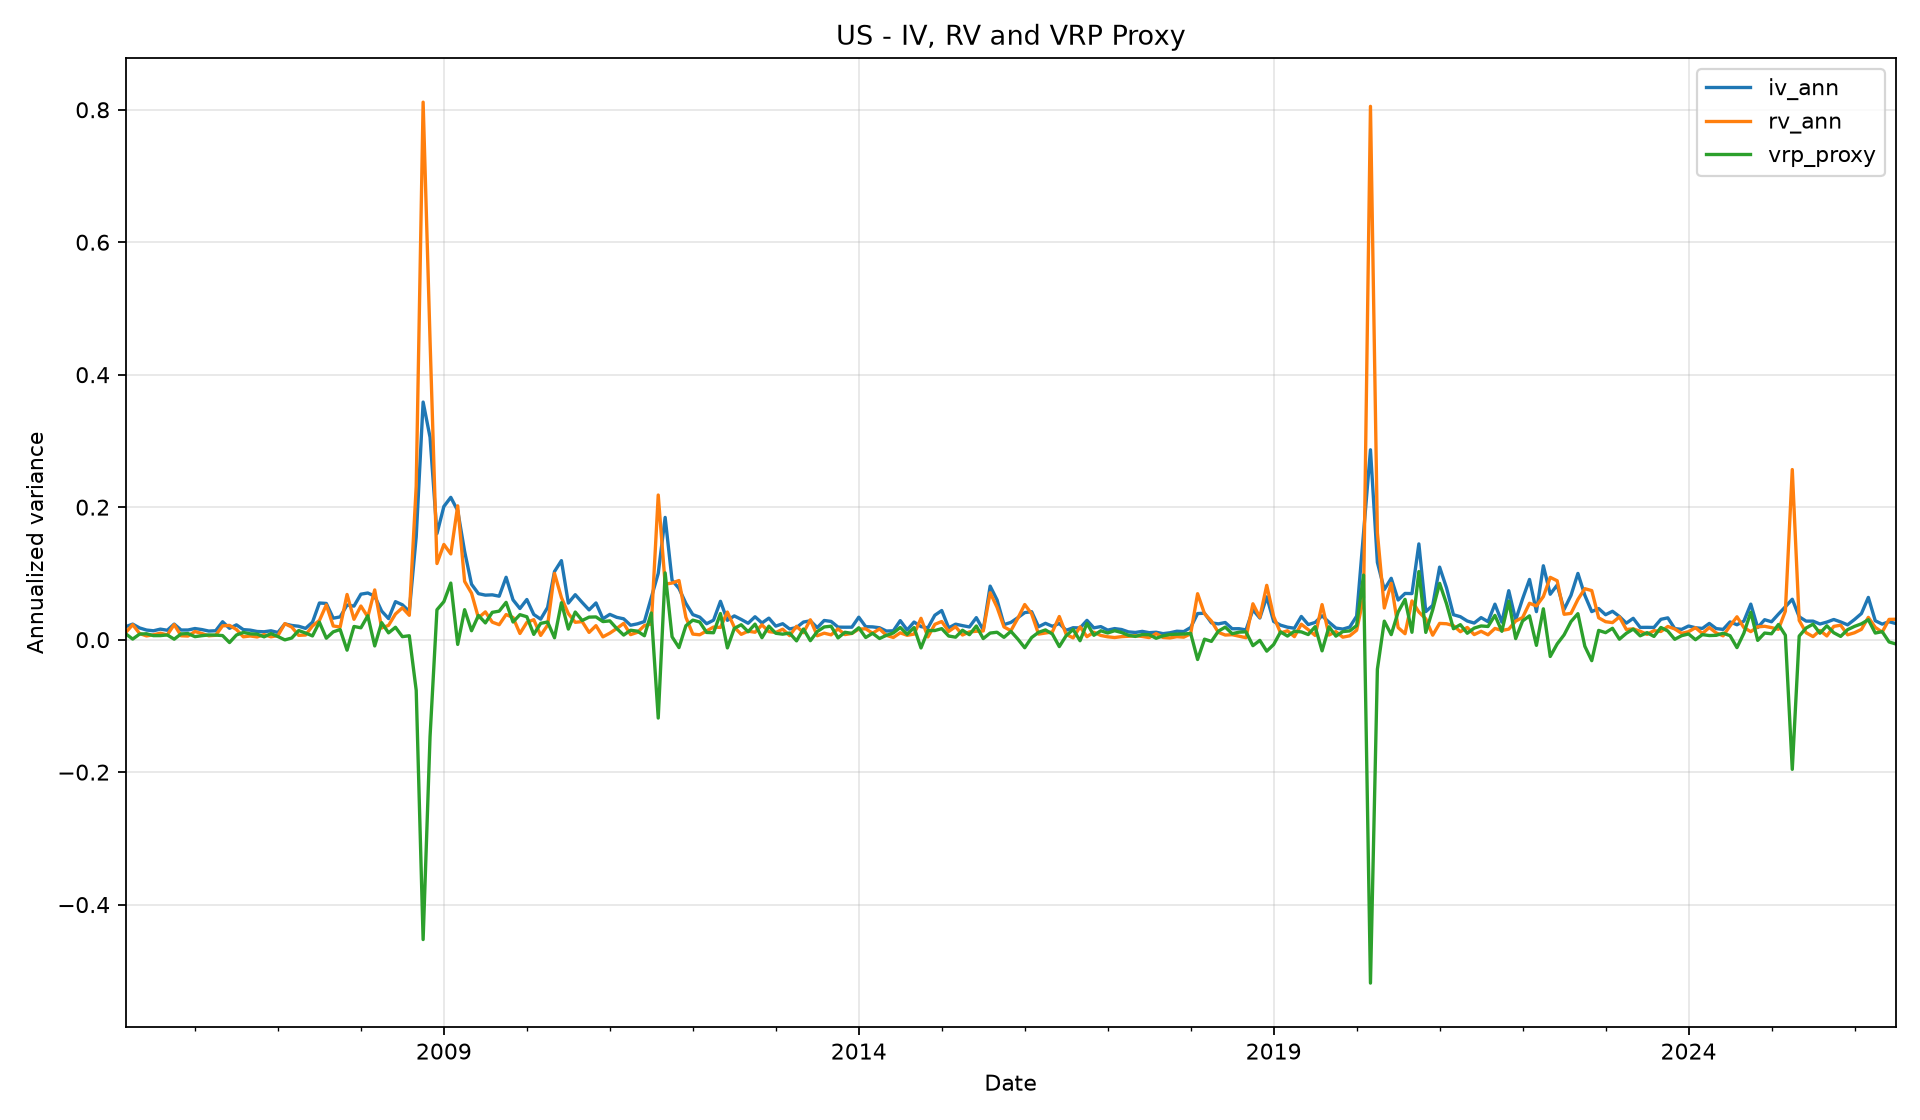
\includegraphics[
    width=\linewidth
]{us_mvp1_vrp_components.png}
\caption{United States}
\end{subfigure}
\hfill
\begin{subfigure}[t]{0.49\textwidth}
\centering
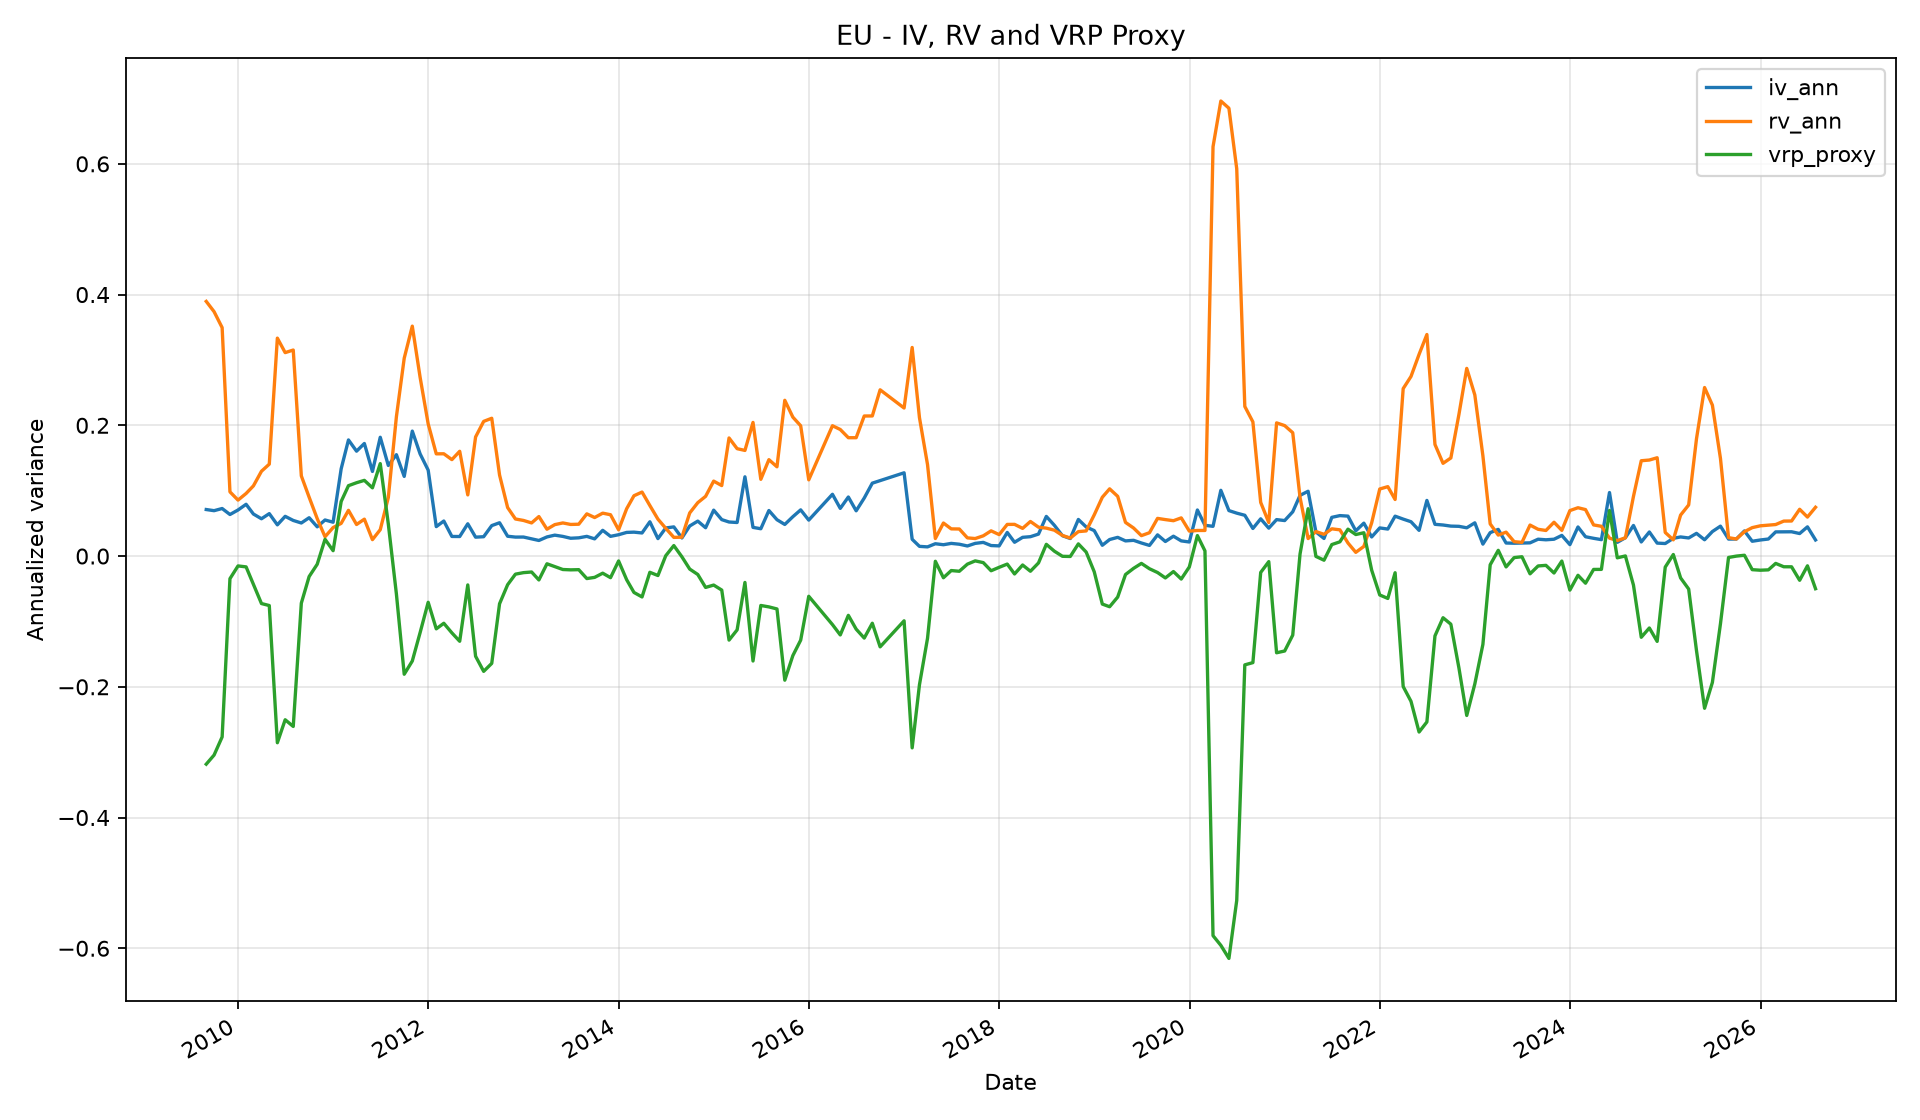
\includegraphics[
    width=\linewidth
]{eu_mvp1_vrp_components.png}
\caption{Europe}
\end{subfigure}

\caption{Implied variance, realized variance, and empirical VRP components}
\label{fig:vrp-components}
\end{figure}

Before turning to the summary statistics, Figure~\ref{fig:allocation-cumulative} displays the cumulative paths of the final implementable allocation comparisons in both markets. Presenting the strategy paths first provides a visual description of relative performance and drawdown behavior before the numerical tables are considered.

\begin{figure}[htbp]
\centering

\begin{subfigure}[t]{0.49\textwidth}
\centering
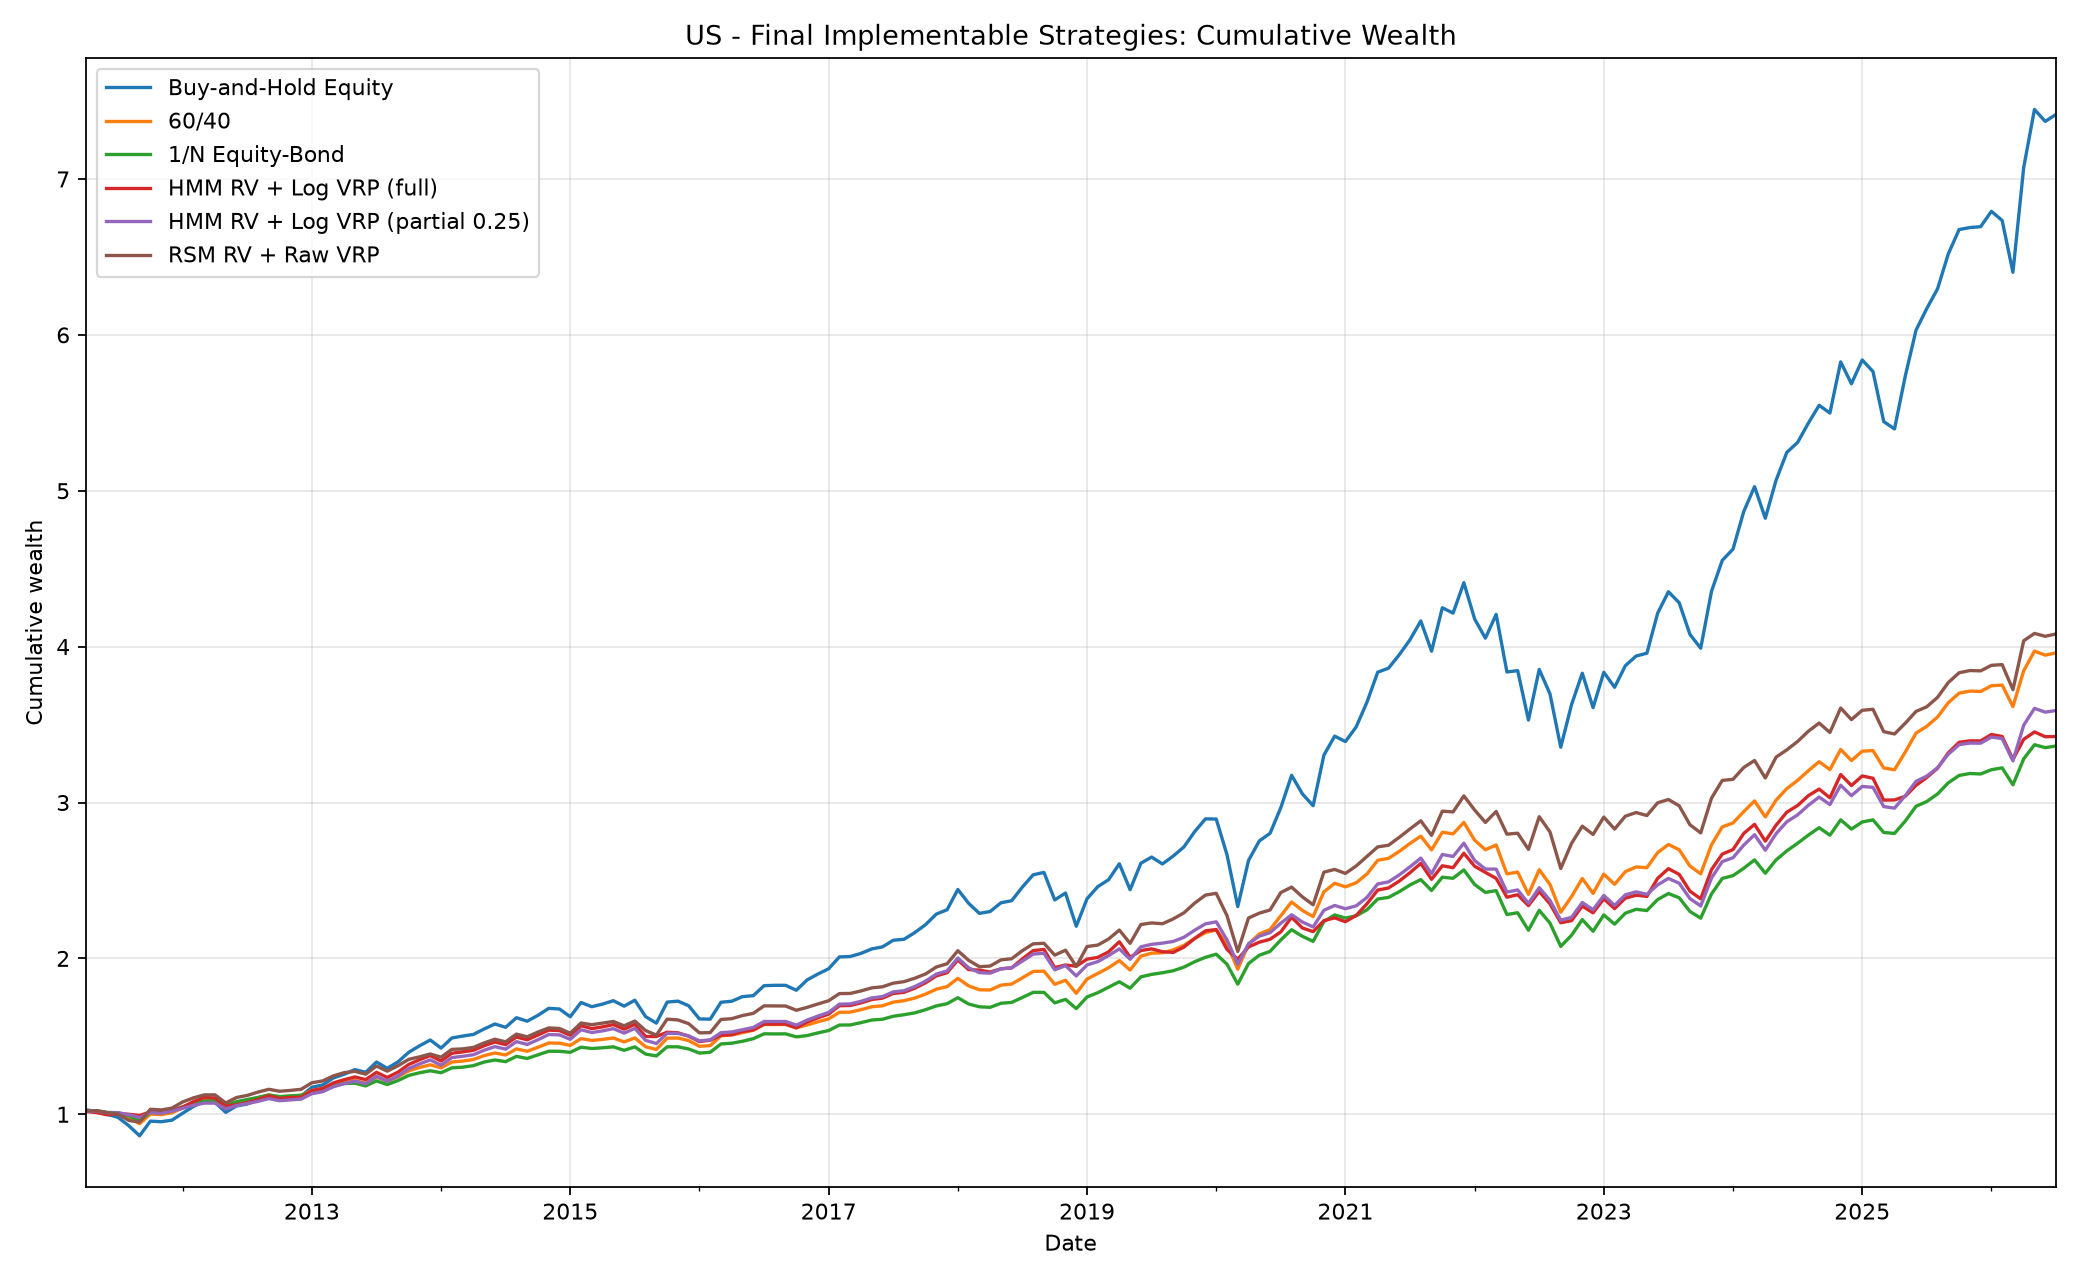
\includegraphics[
    width=\linewidth
]{us_final_implementable_cumulative_returns.png}
\caption{United States}
\end{subfigure}
\hfill
\begin{subfigure}[t]{0.49\textwidth}
\centering
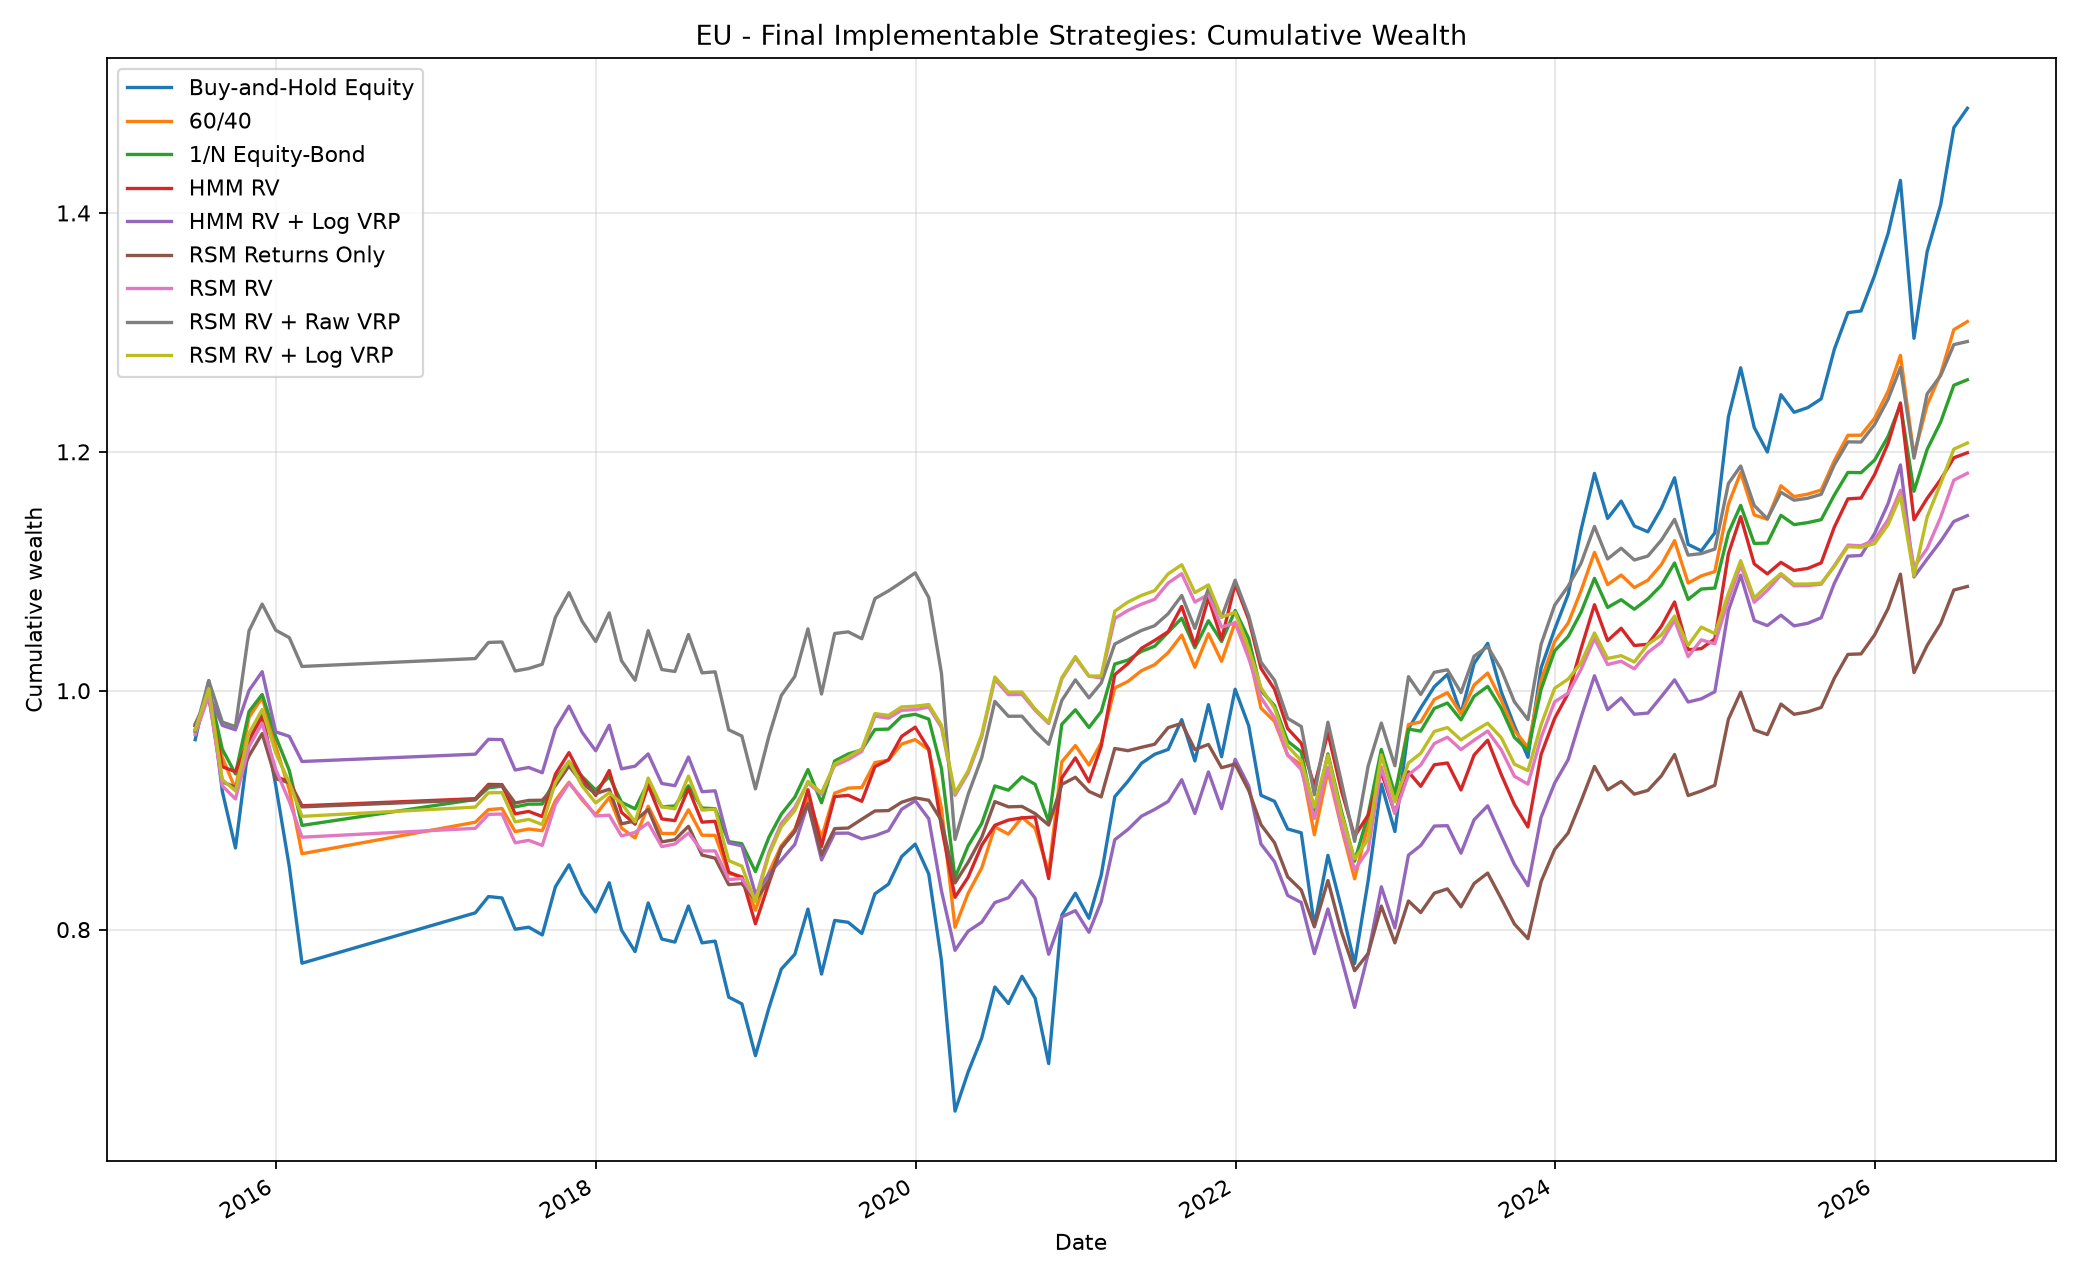
\includegraphics[
    width=\linewidth
]{eu_final_implementable_cumulative_returns.png}
\caption{Europe}
\end{subfigure}

\caption{Cumulative performance of the final implementable allocation comparisons}
\label{fig:allocation-cumulative}
\end{figure}


Figure~\ref{fig:historical-equity-indices} provides complementary market context by showing
the cumulative evolution of the equity components used in the allocation exercise. Each series
is normalized to 100 at the beginning of its corresponding out-of-sample allocation period.
The figure is descriptive: because the United States and European allocation samples begin at
different dates, the two normalized paths should not be interpreted as a common-period
performance comparison.

\begin{figure}[htbp]
\centering
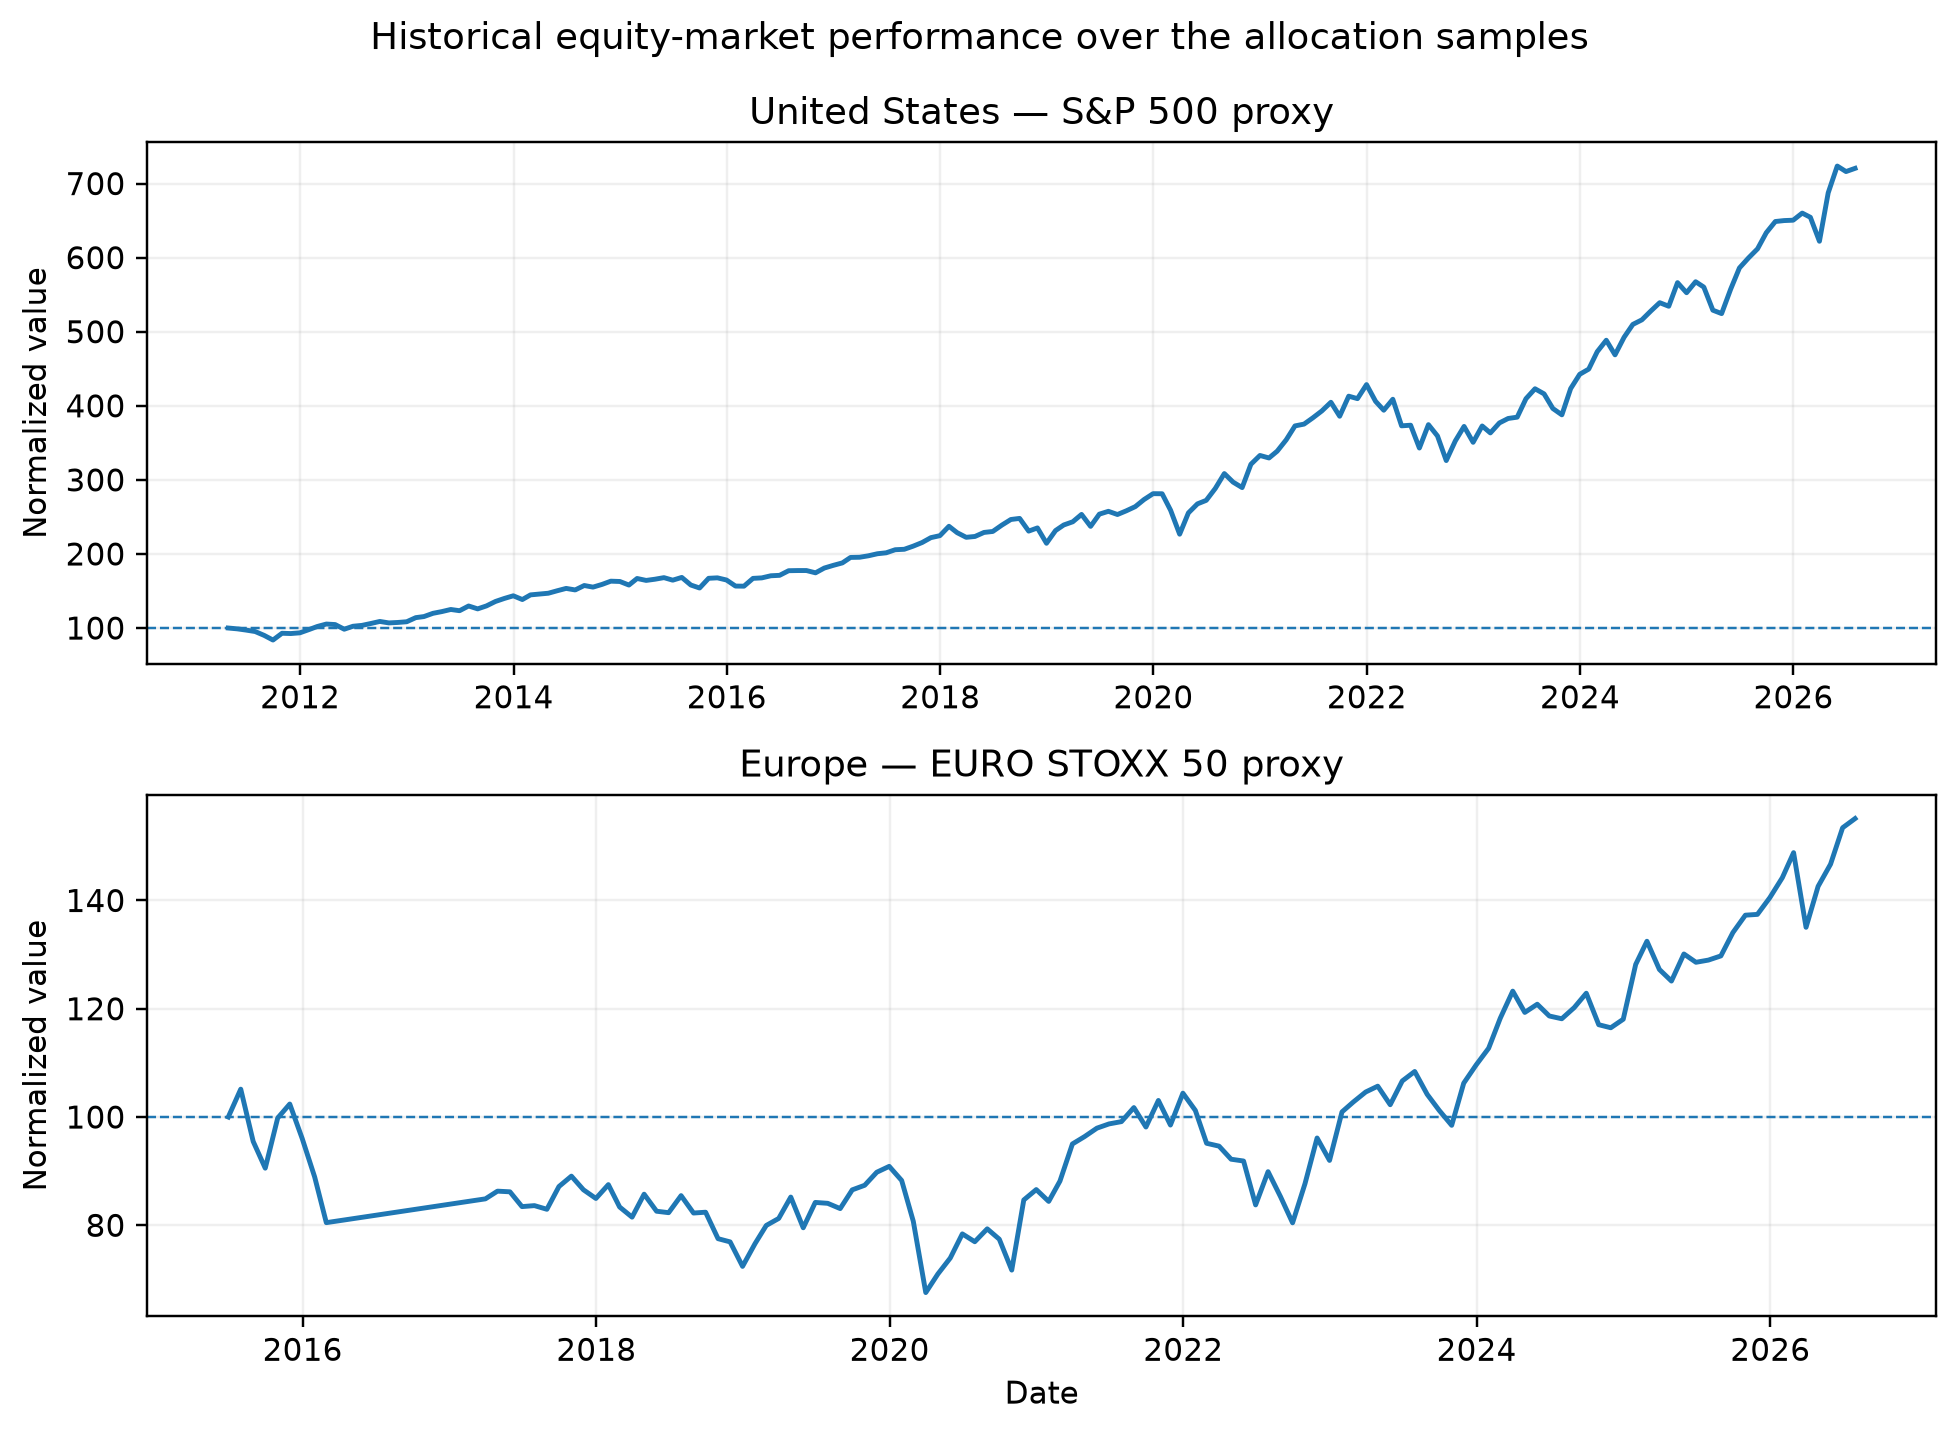
\includegraphics[
    width=0.88\textwidth
]{historical_equity_indices.png}
\caption{Historical evolution of the equity-market components used in the allocation exercise}
\label{fig:historical-equity-indices}
\end{figure}

\subsection{Equity--bond allocation: United States}

Table~\ref{tab:us_allocation} reports the principal United States allocation results. Buy-and-hold equity generates the highest annualized return, at 13.96\%, but also the highest volatility and the largest drawdown among the benchmark portfolios. The 60/40 and equal-weighted portfolios reduce risk substantially. Their Sharpe ratios, 1.024 and 1.025 respectively, provide demanding benchmarks for the dynamic models.

\begin{table}[htbp]
\centering
\small
\caption{United States allocation results}
\label{tab:us_allocation}
\begin{tabularx}{\textwidth}{Xrrrrrr}
\toprule
Strategy
& Return
& Vol.
& Sharpe
& MDD
& CVaR
& Turnover \\
\midrule
Buy-and-Hold Equity
& 13.96\%
& 14.20\%
& 0.995
& -23.93\%
& -8.18\%
& 0.00\% \\
60/40
& 9.39\%
& 9.21\%
& 1.024
& -20.06\%
& -5.20\%
& 1.47\% \\
1/N Equity--Bond
& 8.23\%
& 8.05\%
& 1.025
& -19.10\%
& -4.58\%
& 1.53\% \\
HMM RV + Log VRP
& 8.36\%
& 8.24\%
& 1.019
& -16.67\%
& -4.86\%
& 25.35\% \\
RSM RV + Raw VRP
& 9.61\%
& 10.25\%
& 0.949
& -15.43\%
& -5.53\%
& 36.69\% \\
ML Logistic Base
& 7.58\%
& 7.60\%
& 1.002
& -18.54\%
& -4.35\%
& 17.39\% \\
\bottomrule
\end{tabularx}
\end{table}

The strongest HMM by Sharpe ratio is HMM RV + Log VRP, with a Sharpe ratio of 1.019. This is close to the balanced benchmarks but remains below both 60/40 and equal weighting. Its main improvement is on downside risk: maximum drawdown falls to -16.67\%, compared with -20.06\% for 60/40, -19.10\% for equal weighting, and -23.93\% for buy-and-hold equity.

That improvement is not free. Average turnover rises to 25.35\%, compared with approximately 1.5\% for the static balanced portfolios. The HMM RV + Raw VRP specification produces a higher annualized return of 10.67\% and a Sharpe ratio of 1.014, but does not improve the broad risk-adjusted ranking.

The strongest RSM specification is RSM RV + Raw VRP. Its maximum drawdown of -15.43\% is the smallest among the principal United States allocation strategies, but its Sharpe ratio is only 0.949 and average turnover reaches 36.69\%. The reduction in drawdown is therefore accompanied by substantially greater implementation intensity.

The strongest machine-learning allocation is ML Logistic Base, with a Sharpe ratio of 1.002. Importantly, this leading United States ML specification does not contain the VRP-enhanced feature set. The United States evidence therefore does not support a general claim that adding VRP variables improves allocation performance.

Taken together, the United States allocation results indicate that the dynamic models can alter the distribution of portfolio risk, particularly drawdown, without establishing robust dominance over simple balanced portfolios. The distinction between a better downside statistic and a better investment strategy is economically important.

The implementation mechanism of the selected United States HMM is illustrated in Figure~\ref{fig:hmm-mechanism}. The first panel reports the filtered stress probabilities and the second reports the corresponding equity weights. The figure shows how changes in the inferred latent state are mapped into portfolio exposure rather than treating the HMM as a purely statistical classification device.

\begin{figure}[htbp]
\centering

\begin{subfigure}[t]{0.49\textwidth}
\centering
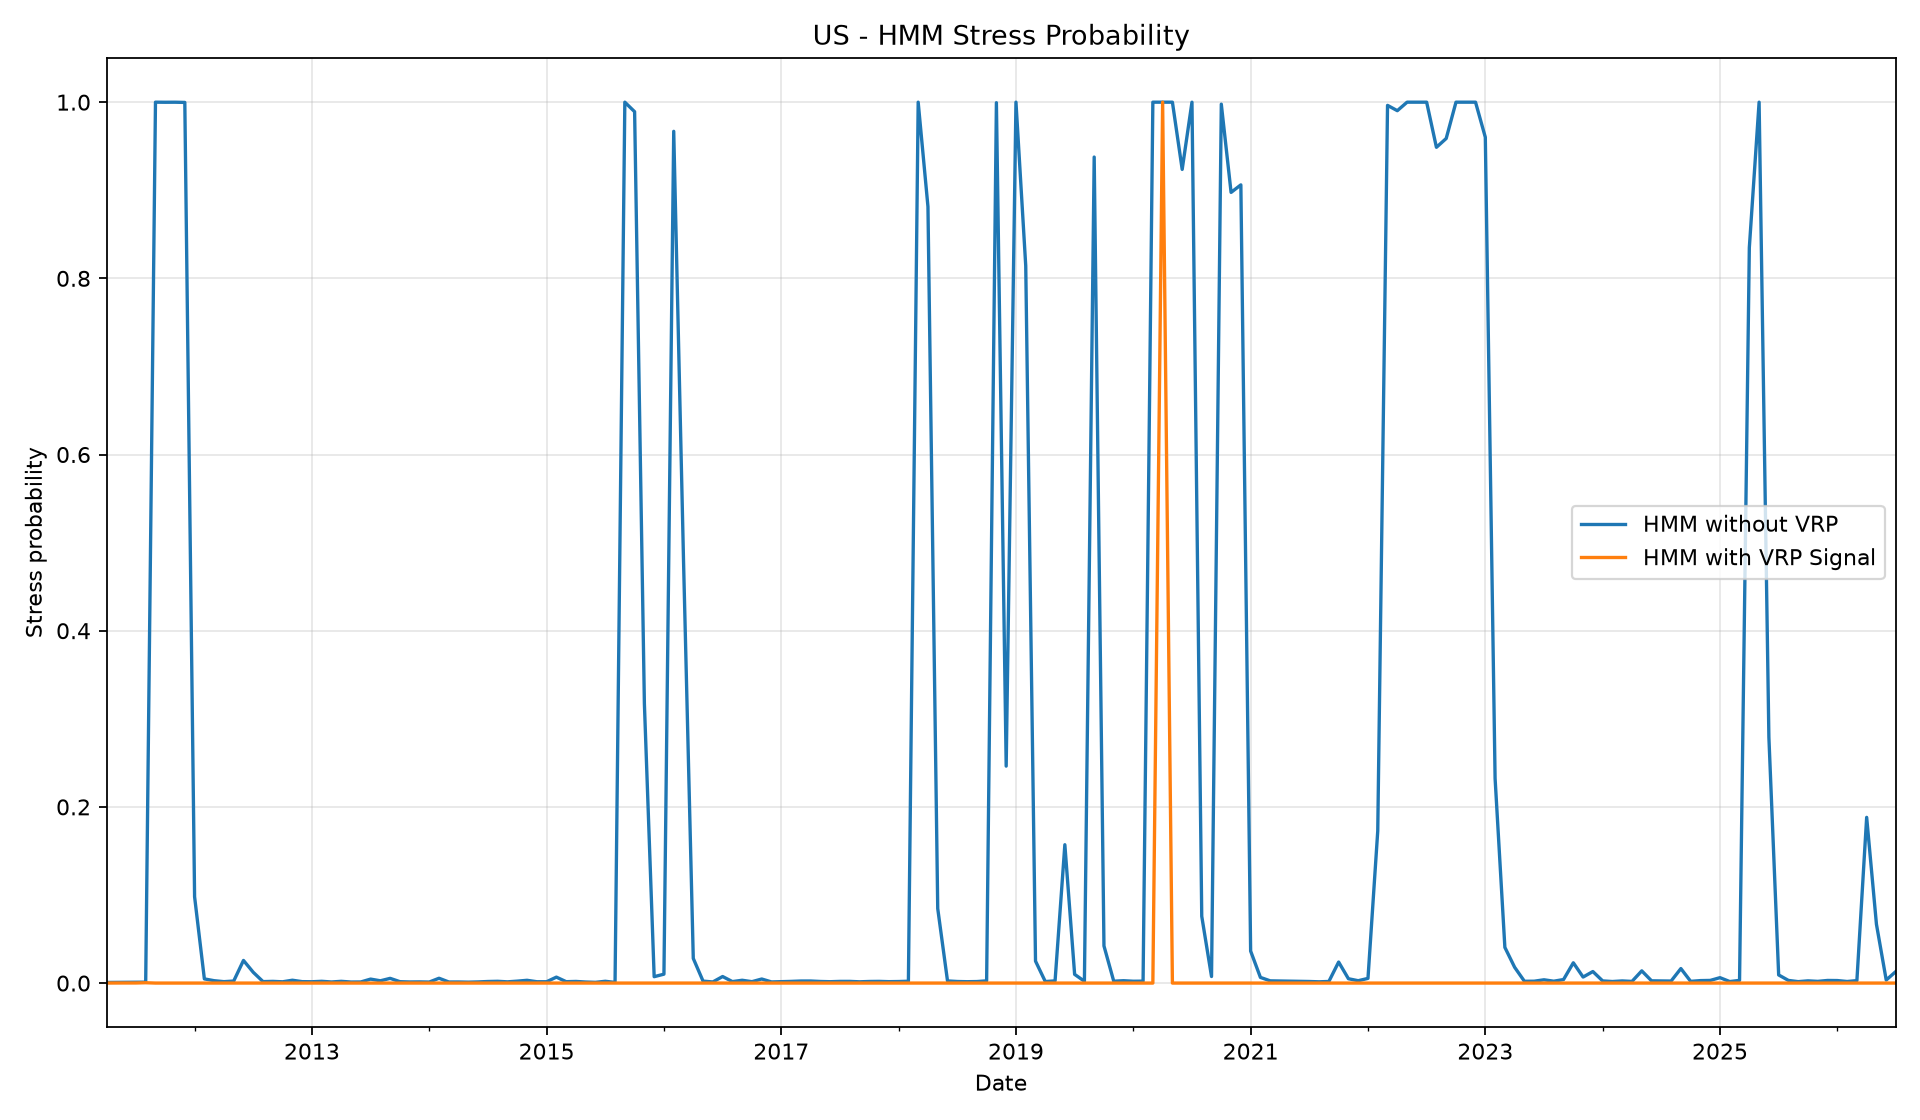
\includegraphics[
    width=\linewidth
]{us_mvp2_hmm_stress_probabilities.png}
\caption{Filtered stress probabilities}
\end{subfigure}
\hfill
\begin{subfigure}[t]{0.49\textwidth}
\centering
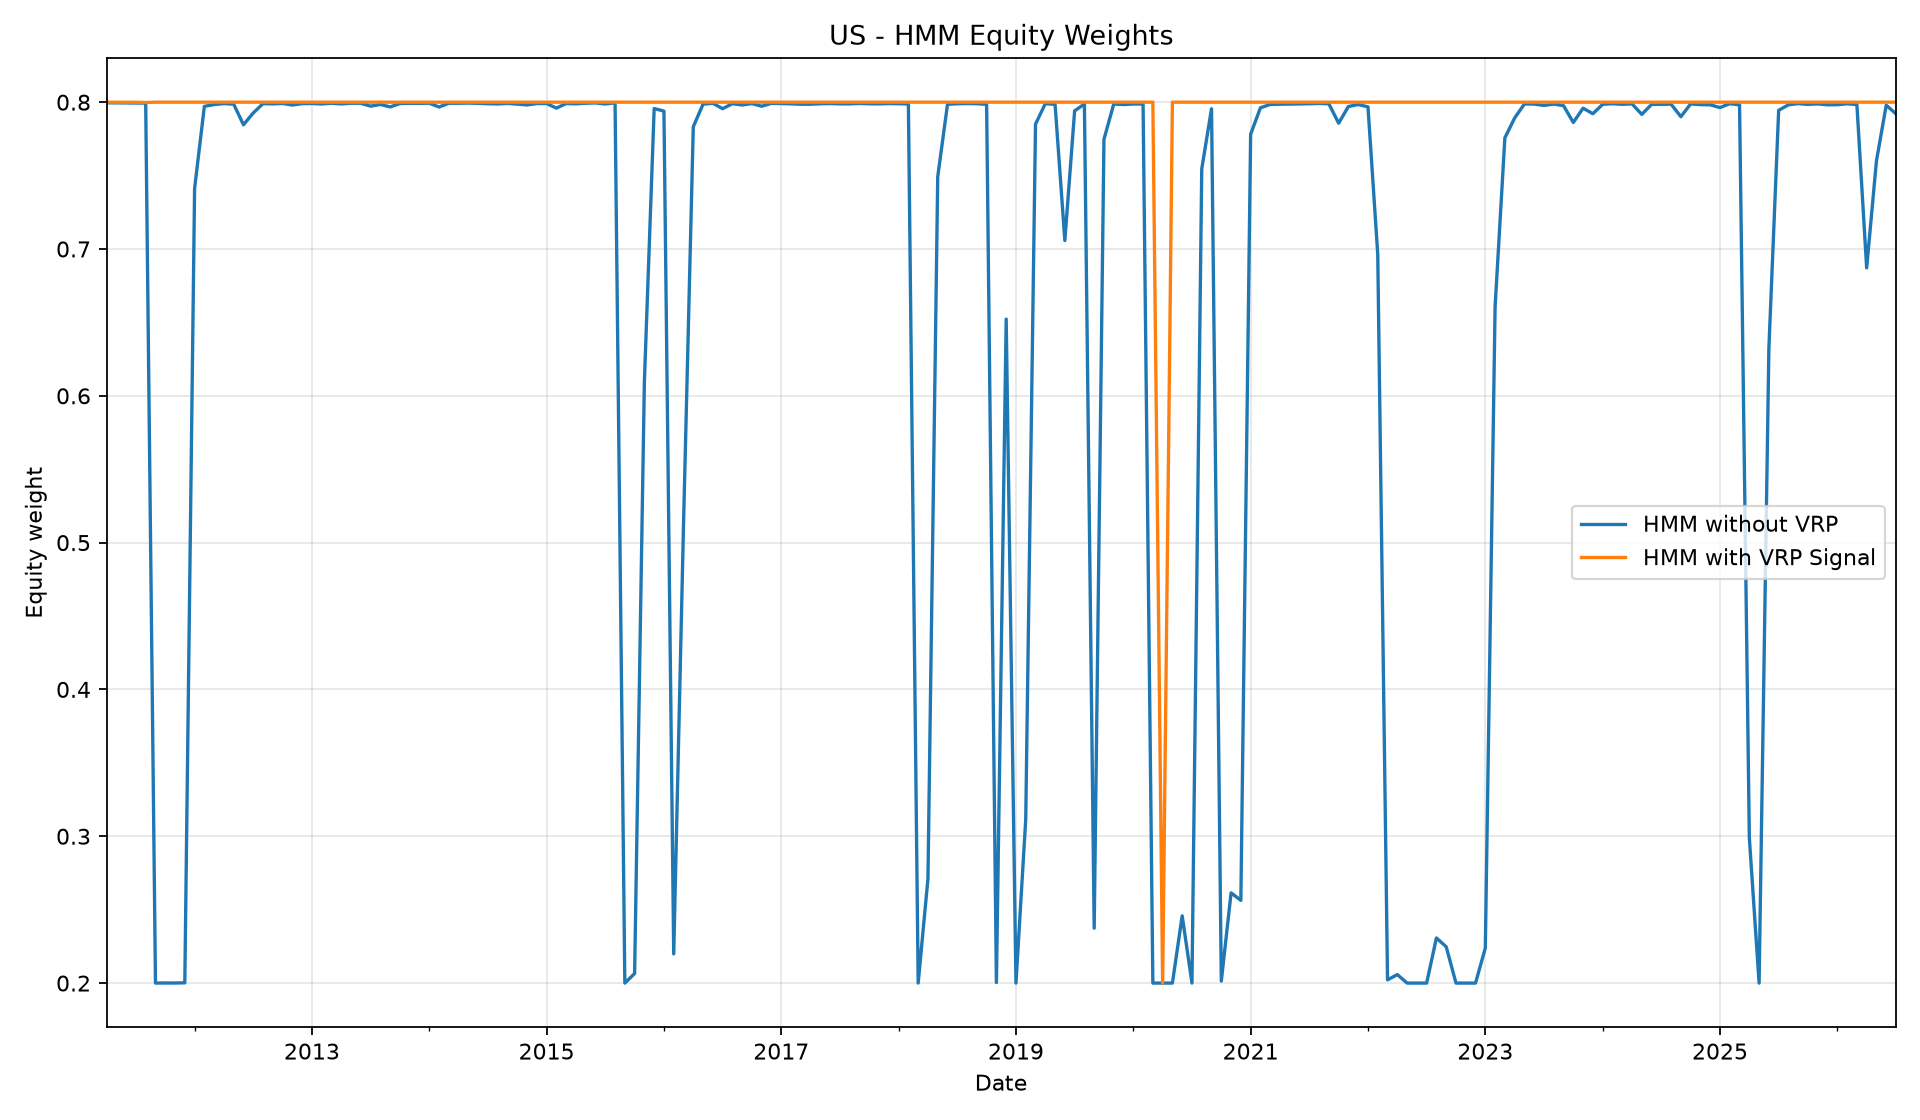
\includegraphics[
    width=\linewidth
]{us_mvp2_hmm_equity_weights.png}
\caption{Resulting equity weights}
\end{subfigure}

\caption{Selected United States HMM: state probability and portfolio mapping}
\label{fig:hmm-mechanism}
\end{figure}

\subsection{Equity--bond allocation: Europe}

The European results are materially weaker in absolute risk-adjusted terms. Table~\ref{tab:eu_allocation} reports the principal comparison.

\begin{table}[htbp]
\centering
\small
\caption{European allocation results}
\label{tab:eu_allocation}
\begin{tabularx}{\textwidth}{Xrrrrrr}
\toprule
Strategy
& Return
& Vol.
& Sharpe
& MDD
& CVaR
& Turnover \\
\midrule
Buy-and-Hold Equity
& 3.98\%
& 17.17\%
& 0.313
& -35.74\%
& -9.86\%
& 0.00\% \\
60/40
& 2.68\%
& 11.24\%
& 0.292
& -20.32\%
& -6.55\%
& 1.74\% \\
1/N Equity--Bond
& 2.30\%
& 9.84\%
& 0.280
& -19.66\%
& -5.85\%
& 1.81\% \\
HMM RV
& 1.80\%
& 10.94\%
& 0.218
& -19.39\%
& -6.20\%
& 17.76\% \\
RSM RV + Raw VRP
& 2.55\%
& 11.24\%
& 0.281
& -20.47\%
& -6.74\%
& 34.00\% \\
ML Random Forest + VRP
& 2.26\%
& 9.99\%
& 0.274
& -19.17\%
& -5.82\%
& 15.38\% \\
\bottomrule
\end{tabularx}
\end{table}

Buy-and-hold equity produces the highest benchmark Sharpe ratio, at 0.313, while the balanced portfolios substantially reduce drawdown. The 60/40 portfolio reaches a Sharpe ratio of 0.292 and equal weighting 0.280.

The strongest HMM is HMM RV, with a Sharpe ratio of 0.218. Adding raw VRP reduces the HMM Sharpe ratio to 0.166, while adding LogVRP produces 0.179. Turnover also increases. Within this model family, the corrected European evidence therefore provides no performance improvement from adding VRP.

The strongest RSM is RSM RV + Raw VRP. Its Sharpe ratio of 0.281 is essentially equal to the equal-weighted benchmark but below both 60/40 and buy-and-hold equity. Average turnover is 34.00\%, compared with less than 2\% for the two balanced benchmarks. Raw VRP therefore contributes useful state information within this specification, but not enough to establish economic dominance.

The strongest European machine-learning allocation is ML Random Forest + VRP. It generates a Sharpe ratio of 0.274 and a maximum drawdown of -19.17\%. The corresponding classifier provides some evidence of incremental predictive information: ROC-AUC is approximately 0.619, precision--recall AUC 0.468, and the Brier score 0.215. However, the portfolio remains below the benchmark Sharpe ratios.

This distinction between prediction and portfolio value is reinforced by the welfare results for the European ML layer. At a risk-aversion coefficient of five, its mean--variance certainty-equivalent advantage is only about 12 basis points relative to 60/40 and approximately -10 basis points relative to equal weighting, with confidence intervals that include zero. Statistical predictability therefore does not translate into robust investor-welfare dominance.

The European allocation conclusion is consequently narrow. VRP-related variables are not empirically absent, and they can contribute information in selected RSM and machine-learning specifications. They do not, however, produce robust superiority in the tested equity--bond allocation framework.

\subsection{Cross-market allocation evidence}

The cross-market allocation evidence rejects a simple interpretation in which greater model complexity automatically creates economic value. In the United States, the strongest dynamic models are close to the balanced benchmarks and sometimes improve drawdown, but they require considerably more turnover. In Europe, the regime and machine-learning models remain below the strongest traditional benchmarks.

The role of VRP is also model dependent. HMM RV + Log VRP is the strongest HMM in the United States, whereas the strongest European HMM excludes VRP. Raw VRP improves the relative ranking of the RSM family in both markets, but neither RSM becomes a dominant allocation strategy. The leading United States ML specification excludes VRP, while the leading European ML specification includes it.

The allocation layer therefore provides evidence that variance information can affect estimated states and selected portfolio-risk characteristics, but it does not establish a universal allocation premium.



\subsection{Underlying direct variance-payoff diagnostics}

The second evidence layer begins with the modeled short-variance payoff itself. Table~\ref{tab:payoff_diag} summarizes the underlying settlement observations before the final strategy alignment.

\begin{table}[htbp]
\centering
\small
\caption{Underlying short-variance payoff diagnostics}
\label{tab:payoff_diag}
\begin{tabularx}{\textwidth}{Xrrrrrr}
\toprule
Market
& Obs.
& Positive
& Mean norm.
& Skew
& 1\% quantile
& Worst \\
\midrule
United States
& 256
& 82.42\%
& 0.253
& -3.849
& -4.080
& -4.432 \\
Europe
& 194
& 78.35\%
& 0.239
& -2.231
& -2.060
& -2.439 \\
\bottomrule
\end{tabularx}
\end{table}

The average variance strike is 4.35\% in the United States and 5.22\% in Europe, compared with average realized variance of 3.57\% and 4.02\%, respectively. The corresponding mean short-variance spreads are positive in both markets.

Positive carry is frequent but not symmetric. The normalized payoff is positive in 82.42\% of United States observations and 78.35\% of European observations. At the same time, skewness is strongly negative: -3.849 in the United States and -2.231 in Europe. Approximately 4.69\% of United States observations and 4.12\% of European observations generate normalized losses below -100\%.

These diagnostics are central to interpretation. A high positive-payoff frequency does not imply an arbitrage or a low-risk return process. The short-variance mechanism earns frequent positive carry while remaining exposed to infrequent, disproportionately large losses. Risk targeting, exposure constraints and welfare analysis are therefore necessary before drawing an economic conclusion.

\subsection{United States direct-variance evidence}

The selected United States direct-variance specification is the 10\% annual-volatility target activated by the High-VRP gate. Table~\ref{tab:direct_main} reports the selected direct strategies for both markets.

\begin{table}[htbp]
\centering
\small
\caption{Selected model-based direct variance-payoff strategies}
\label{tab:direct_main}
\begin{tabularx}{\textwidth}{Xrrrrrrrr}
\toprule
Market / strategy
& Return
& Vol.
& Sharpe
& Sortino
& MDD
& CVaR
& Turn.
& Obs. \\
\midrule
US High VRP
& 6.23\%
& 7.17\%
& 0.882
& 1.218
& -23.46\%
& -5.26\%
& 2.01\%
& 232 \\
EU VRP $>0$
& 13.08\%
& 9.70\%
& 1.324
& 1.891
& -21.36\%
& -7.34\%
& 4.39\%
& 170 \\
\bottomrule
\end{tabularx}
\end{table}

The United States High-VRP strategy generates an annualized return of 6.23\%, volatility of 7.17\%, and a Sharpe ratio of 0.882. Its maximum drawdown is -23.46\% and its empirical 95\% CVaR is -5.26\%.

On the same 232-observation direct-variance comparison sample, the 60/40 benchmark has a Sharpe ratio of 0.827 and equal weighting 0.852. The direct strategy therefore improves the Sharpe ratio on this particular aligned sample. This difference is not sufficient to establish investor-welfare dominance.

The alternative United States strategy active whenever lagged VRP is positive illustrates the importance of the exposure rule. It produces an annualized return of 8.18\%, but volatility rises to 16.07\%, the Sharpe ratio falls to 0.590, maximum drawdown reaches -39.77\%, and CVaR reaches -13.29\%. Selecting months with unusually high lagged VRP therefore produces a materially more defensive United States payoff profile than merely requiring VRP to be positive.

\subsection{European direct-variance evidence}

The European result is considerably stronger within the tested approximation. The selected strategy takes exposure when lagged VRP is positive. It produces an annualized return of 13.08\%, annualized volatility of 9.70\%, a Sharpe ratio of 1.324, and a Sortino ratio of 1.891. Maximum drawdown is -21.36\% and empirical 95\% CVaR is -7.34\%.

This result is economically different from the European allocation evidence. Adding VRP to HMM, RSM, or machine-learning allocation does not generate robust benchmark dominance. Yet mapping lagged implied variance into the model-based short-variance payoff produces substantially stronger risk-adjusted performance.

This is the first central cross-channel result of the thesis: weak evidence for VRP as a universal allocation feature does not imply weak variance carry. Information value and payoff value are distinct empirical objects.

The result must nevertheless retain the methodological qualification established earlier. The strategy is a model-based direct variance-payoff approximation. It is not an observed variance-swap return and does not include an exact option-replicated strike, contractual variance notional, collateral and margin processes, dealer bid--ask spreads, or daily mark-to-market.

Figure~\ref{fig:direct-variance-cross-market} summarizes the central cross-market direct-payoff result. Panel (a) compares the Sharpe ratio of the selected direct-variance strategy with the two balanced benchmarks. Panel (b) reports the corresponding fee-equivalent welfare difference at $\gamma=5$. The two panels highlight why Sharpe-ratio improvement alone is insufficient for the United States conclusion, while the European result remains economically much stronger under the welfare criterion.

\begin{figure}[htbp]
\centering

\begin{subfigure}[t]{0.49\textwidth}
\centering
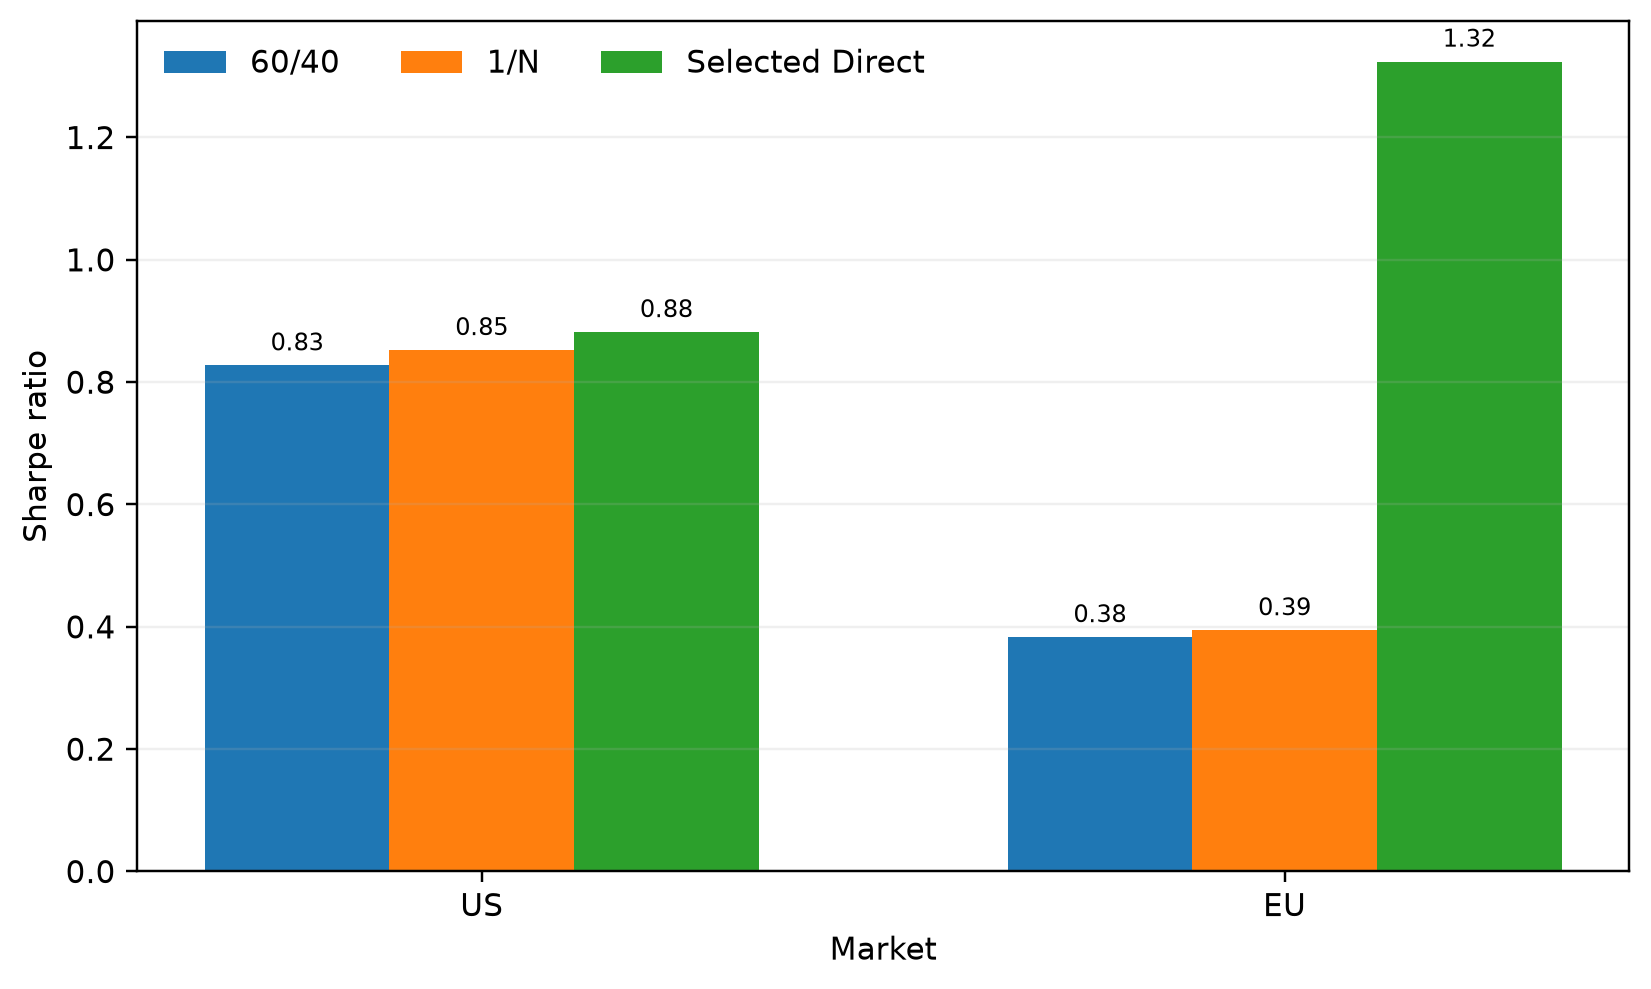
\includegraphics[
    width=\linewidth
]{direct_variance_sharpe_cross_market.png}
\caption{Sharpe-ratio comparison}
\end{subfigure}
\hfill
\begin{subfigure}[t]{0.49\textwidth}
\centering
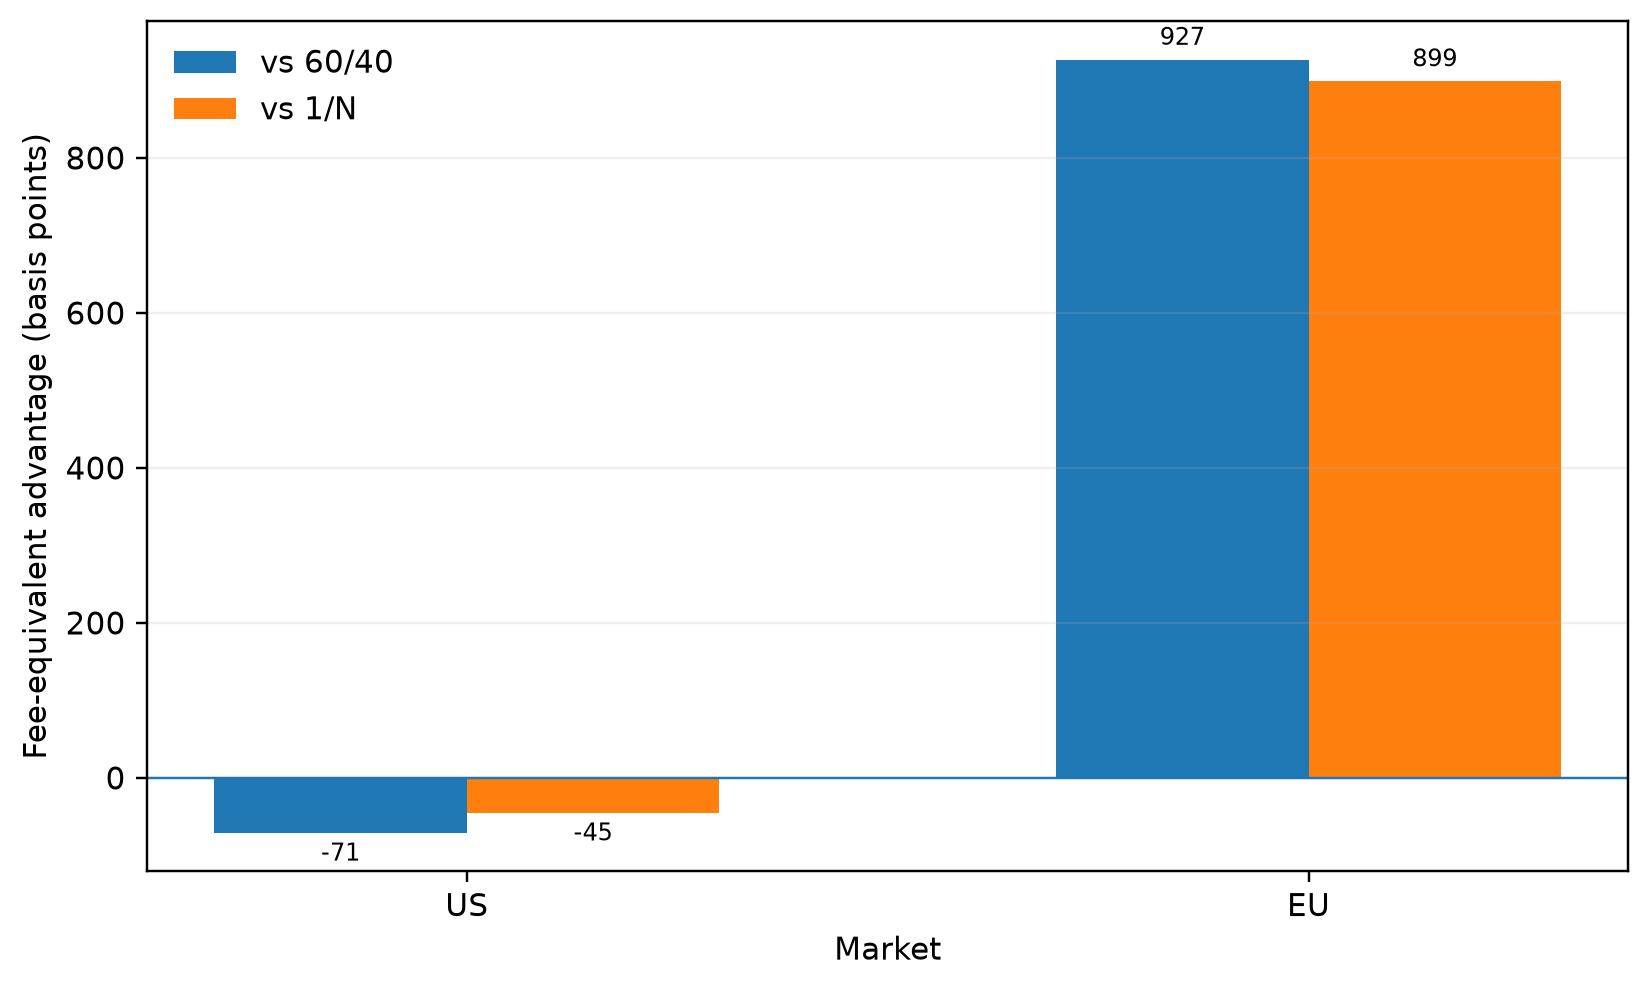
\includegraphics[
    width=\linewidth
]{direct_variance_welfare_cross_market.png}
\caption{Fee-equivalent welfare comparison}
\end{subfigure}

\caption{Cross-market economic comparison of the selected model-based direct variance-payoff strategies}
\label{fig:direct-variance-cross-market}
\end{figure}

\subsection{Investor-welfare evidence}

Risk-adjusted performance alone does not establish economic superiority, particularly for negatively skewed strategies. Table~\ref{tab:welfare_main} therefore reports the principal welfare comparison at risk aversion $\gamma=5$.

\begin{table}[htbp]
\centering
\small
\caption{Direct-variance welfare evidence at $\gamma=5$}
\label{tab:welfare_main}
\begin{tabularx}{\textwidth}{Xrrrrrr}
\toprule
Strategy
& MV CEQ
& CRRA CE
& vs 60/40
& CI low
& vs 1/N
& CI low \\
\midrule
US High VRP
& 5.04\%
& 5.00\%
& -70.9 bp
& -5.49\%
& -45.0 bp
& -4.94\% \\
EU VRP $>0$
& 10.49\%
& 10.67\%
& +926.6 bp
& +3.27\%
& +898.8 bp
& +2.91\% \\
\bottomrule
\end{tabularx}
\end{table}

The United States conclusion weakens once investor welfare is considered. The High-VRP strategy has an annualized mean--variance certainty equivalent of 5.04\% and a CRRA certainty equivalent of 5.00\%. Its mean--variance welfare difference is -70.9 basis points relative to 60/40 and -45.0 basis points relative to equal weighting. The bootstrap intervals include zero: the interval relative to 60/40 runs from approximately -5.49\% to +4.92\%, while the interval relative to equal weighting runs from -4.94\% to +4.59\%. The United States direct strategy therefore does not establish statistically robust welfare dominance.

The European result is materially different. The VRP-positive strategy has a mean--variance certainty equivalent of 10.49\% and a CRRA certainty equivalent of 10.67\%. Its mean--variance advantage is 926.6 basis points relative to 60/40 and 898.8 basis points relative to equal weighting. More importantly, the lower bootstrap bounds remain positive at +3.27\% and +2.91\%, respectively.

The European evidence therefore survives a more demanding economic criterion than the Sharpe ratio alone. Within the tested direct-payoff approximation, the selected European strategy produces positive investor-welfare differences against both traditional portfolios and those differences remain positive at the lower bootstrap bounds.

\subsection{Empirical synthesis}

Three findings emerge from the combined evidence.

First, the allocation channel is economically modest. In the United States, the best HMM, RSM, and machine-learning specifications are competitive in selected dimensions but do not dominate the traditional portfolios. The most visible benefit is sometimes lower drawdown, obtained at the cost of substantially higher turnover. In Europe, the evidence is weaker: the strongest dynamic models remain below the strongest benchmark Sharpe ratios.

Second, predictive information and investment value are not equivalent. European Random Forest results indicate that VRP variables contain incremental stress-classification information, yet this improvement does not generate statistically significant allocation welfare. The same distinction appears across the regime models, where adding VRP changes state probabilities and model rankings without producing robust portfolio dominance.

Third, the payoff channel produces the strongest cross-market asymmetry. The United States direct-variance strategy has attractive defensive characteristics but does not establish robust welfare superiority. In Europe, the selected direct variance-payoff approximation generates a Sharpe ratio of 1.324 and large positive certainty-equivalent differences with positive lower bootstrap bounds.

The results therefore do not support the statement that VRP is universally more useful as a state variable, nor do they support a claim that VRP fails in Europe. Instead, they imply that the economic value associated with variance information depends critically on the payoff structure through which it is harvested.

The next section tests whether these conclusions survive changes in implementation assumptions, risk-estimation windows, exposure limits, subperiods, crisis exclusions, rebalancing rules, and investor risk aversion.


\section{Robustness and Implementation}
\label{sec:robustness}

The purpose of the robustness analysis is not to search retrospectively for the calibration with the highest historical performance. It is to determine whether the conclusions reported in the previous section survive economically plausible changes in implementation, risk estimation, exposure limits, sample composition, and investor preferences.

The two empirical channels require different tests. Dynamic equity--bond allocation is primarily exposed to turnover, model instability, and the cost of responding to changing estimated state probabilities. The model-based direct variance-payoff approximation is additionally exposed to monthly roll costs, negatively skewed payoff shocks, errors in lagged risk estimation, notional constraints, and the concentration of returns in particular market episodes.

All sensitivity comparisons preserve the timing rules described in the methodology. Direct-variance parameter grids are aligned to a common sample within each sensitivity dimension. Consequently, a 12-month and a 60-month risk-estimation specification are compared only over dates available to both. Appendix B summarizes the parameter grid and supplementary robustness diagnostics, while the full machine-readable grids are retained under \texttt{outputs/tables/}; the main text focuses on the results required to assess the economic conclusion.

\subsection{Allocation implementation robustness}

The principal allocation models require substantially more trading than the static benchmarks. In the United States allocation sample, average turnover is 1.47\% for 60/40 and 1.53\% for equal weighting, compared with 25.35\% for HMM RV + Log VRP and 36.69\% for RSM RV + Raw VRP. In Europe, the strongest dynamic specifications similarly require turnover between approximately 15\% and 34\%, compared with less than 2\% for the balanced portfolios.

This implementation burden matters because the gross advantage of the dynamic models is small. Table~\ref{tab:allocation_cost_robustness} shows the transaction-cost sensitivity of the selected United States HMM.

\begin{table}[htbp]
\centering
\small
\caption{United States allocation Sharpe ratios under transaction costs}
\label{tab:allocation_cost_robustness}
\begin{tabular}{lrrr}
\toprule
Cost
& 60/40
& 1/N
& HMM RV + Log VRP \\
\midrule
0 bps
& 1.026
& 1.028
& 1.055 \\
10 bps
& 1.024
& 1.025
& 1.019 \\
25 bps
& 1.021
& 1.022
& 0.963 \\
50 bps
& 1.016
& 1.016
& 0.869 \\
\bottomrule
\end{tabular}
\end{table}

Before transaction costs, the HMM produces a higher Sharpe ratio than the two balanced portfolios. At the 10-basis-point baseline, the ranking reverses. At 25 and 50 basis points, the HMM deteriorates more rapidly because its turnover is much larger. Its drawdown advantage is more persistent than its Sharpe advantage: at baseline costs, maximum drawdown remains -16.67\%, compared with -20.06\% for 60/40 and -19.10\% for equal weighting. The appropriate interpretation is therefore defensive rather than one of broad performance dominance.

A no-trade band produces only a modest improvement. Increasing the band from zero to 10\% raises the selected HMM Sharpe ratio from approximately 1.019 to 1.026 and lowers average turnover from approximately 25.30\% to 23.53\%. Small adjustments are removed, but large changes in estimated state probabilities still require substantial trading.

Partial rebalancing is more effective. Instead of moving fully to the model target each month, the implemented portfolio moves only a fraction of the distance. Table~\ref{tab:partial_rebalancing} compares full rebalancing with an adjustment speed of 0.25.

\begin{table}[htbp]
\centering
\small
\caption{Partial rebalancing of the selected United States HMM}
\label{tab:partial_rebalancing}
\begin{tabularx}{\textwidth}{Xrrrrr}
\toprule
Implementation
& Return
& Vol.
& Sharpe
& MDD
& Turnover \\
\midrule
Full rebalancing
& 8.36\%
& 8.24\%
& 1.019
& -16.67\%
& 25.35\% \\
Partial, $\lambda=0.25$
& 8.69\%
& 8.62\%
& 1.014
& -18.04\%
& 9.10\% \\
\bottomrule
\end{tabularx}
\end{table}

The 0.25 implementation reduces turnover by approximately two thirds while changing the Sharpe ratio only marginally. Maximum drawdown remains below that of 60/40 and buy-and-hold equity. This makes the HMM operationally more plausible, but it does not make it a statistically or economically dominant allocation strategy.

The European allocation conclusion is even less sensitive to implementation choices. The strongest HMM reaches a Sharpe ratio of 0.218, the strongest RSM 0.281, and the strongest machine-learning strategy 0.274. These values remain close to or below the simple benchmarks while requiring materially greater turnover. There is therefore no strong baseline allocation advantage for implementation refinements to preserve.

\subsection{Direct-variance transaction-cost sensitivity}

The direct-variance cost treatment differs from portfolio rebalancing. Each one-month modeled variance exposure settles and a new exposure must be initiated. Costs are therefore charged on the full absolute monthly notional rather than only on the change in notional.

The tested cost rates are 0, 10, 25, and 50 basis points per unit of monthly notional. Table~\ref{tab:direct_costs} reports the complete selected-strategy cost grid.

\begin{table}[htbp]
\centering
\scriptsize
\caption{Direct-variance transaction-cost sensitivity}
\label{tab:direct_costs}
\begin{tabularx}{\textwidth}{Xrrrrrrr}
\toprule
Market / cost
& Return
& Vol.
& Sharpe
& MDD
& MV CEQ
& vs 60/40
& vs 1/N \\
\midrule
US 0 bps
& 6.26\%
& 7.18\%
& 0.885
& -23.42\%
& 5.06\%
& -0.69\%
& -0.43\% \\
US 10 bps
& 6.23\%
& 7.17\%
& 0.882
& -23.46\%
& 5.04\%
& -0.71\%
& -0.45\% \\
US 25 bps
& 6.19\%
& 7.17\%
& 0.877
& -23.53\%
& 5.00\%
& -0.74\%
& -0.48\% \\
US 50 bps
& 6.13\%
& 7.16\%
& 0.869
& -23.63\%
& 4.95\%
& -0.80\%
& -0.54\% \\
EU 0 bps
& 13.14\%
& 9.70\%
& 1.329
& -21.35\%
& 10.54\%
& 9.32\%
& 9.04\% \\
EU 10 bps
& 13.08\%
& 9.70\%
& 1.324
& -21.36\%
& 10.49\%
& 9.27\%
& 8.99\% \\
EU 25 bps
& 12.99\%
& 9.69\%
& 1.316
& -21.38\%
& 10.41\%
& 9.19\%
& 8.91\% \\
EU 50 bps
& 12.84\%
& 9.69\%
& 1.303
& -21.42\%
& 10.28\%
& 9.06\%
& 8.78\% \\
\bottomrule
\end{tabularx}
\end{table}

The selected United States strategy is not highly sensitive to the tested cost range because its average active notional is low. This does not improve the welfare conclusion: its mean--variance certainty-equivalent difference is already negative at zero costs and becomes slightly more negative as costs rise.

The European result is more informative. Even at 50 basis points, the Sharpe ratio remains 1.303 and the annualized mean--variance certainty-equivalent advantage remains 9.06 percentage points relative to 60/40 and 8.78 percentage points relative to equal weighting. The result is therefore not generated by assuming zero or near-zero stylized roll costs. This test does not establish that real derivative implementation costs would lie inside the tested range.

\subsection{Sensitivity to the risk-estimation window}

The baseline payoff-volatility estimate uses a 36-month lookback. Robustness tests consider 12, 24, 36, and 60 months. These specifications are evaluated on the common sample required by the longest window, so the 36-month values in Table~\ref{tab:lookback_robustness} differ slightly from the unrestricted baseline.

\begin{table}[htbp]
\centering
\scriptsize
\caption{Direct-variance risk-estimation-window sensitivity}
\label{tab:lookback_robustness}
\begin{tabularx}{\textwidth}{Xrrrrrrr}
\toprule
Market / window
& Return
& Vol.
& Sharpe
& MDD
& MV CEQ
& vs 60/40
& vs 1/N \\
\midrule
US 12m
& 8.10\%
& 16.15\%
& 0.578
& -50.69\%
& 2.81\%
& -3.30\%
& -2.94\% \\
US 24m
& 6.38\%
& 9.94\%
& 0.678
& -32.59\%
& 4.27\%
& -1.85\%
& -1.49\% \\
US 36m
& 6.50\%
& 7.10\%
& 0.926
& -23.46\%
& 5.32\%
& -0.80\%
& -0.44\% \\
US 60m
& 6.26\%
& 6.87\%
& 0.922
& -23.00\%
& 5.15\%
& -0.97\%
& -0.60\% \\
EU 12m
& 18.35\%
& 11.21\%
& 1.570
& -15.92\%
& 14.45\%
& 11.74\%
& 11.78\% \\
EU 24m
& 15.66\%
& 10.46\%
& 1.453
& -19.97\%
& 12.46\%
& 9.75\%
& 9.79\% \\
EU 36m
& 14.15\%
& 9.79\%
& 1.409
& -21.36\%
& 11.40\%
& 8.69\%
& 8.73\% \\
EU 60m
& 13.92\%
& 8.93\%
& 1.513
& -17.21\%
& 11.52\%
& 8.80\%
& 8.84\% \\
\bottomrule
\end{tabularx}
\end{table}

The United States result is sensitive to short risk-estimation windows. The 12-month specification realizes volatility of 16.15\%, a maximum drawdown of -50.69\%, and a Sharpe ratio of only 0.578. A short history can therefore assign excessive exposure before a large payoff shock. The 36- and 60-month specifications are substantially more stable, although their welfare differences remain negative relative to both benchmarks.

The European conclusion is stable across the entire grid. Every tested window produces a Sharpe ratio above 1.40 on the aligned sample and a large positive certainty-equivalent difference. The strongest ex post calibration is not the object of the test; the important result is that the European conclusion does not depend on a unique volatility lookback.

\subsection{Notional-cap sensitivity}

The maximum absolute notionals tested are 5\%, 10\%, 15\%, 25\%, and 50\%. Caps above 15\% are effectively non-binding for the selected United States strategy, while caps above 10\% are non-binding for the selected European strategy. Table~\ref{tab:cap_robustness} therefore reports the economically informative subset of the grid.

\begin{table}[htbp]
\centering
\small
\caption{Selected notional-cap sensitivity}
\label{tab:cap_robustness}
\begin{tabularx}{\textwidth}{Xrrrrrr}
\toprule
Market / cap
& Return
& Vol.
& Sharpe
& MDD
& MV CEQ
& vs benchmarks \\
\midrule
US 5\%
& 5.37\%
& 6.53\%
& 0.836
& -23.46\%
& 4.39\%
& negative \\
US 10\%
& 6.25\%
& 7.17\%
& 0.884
& -23.46\%
& 5.05\%
& negative \\
US 25\%
& 6.23\%
& 7.17\%
& 0.882
& -23.46\%
& 5.04\%
& negative \\
EU 5\%
& 12.07\%
& 7.94\%
& 1.482
& -17.95\%
& 10.19\%
& positive \\
EU 10\%
& 13.08\%
& 9.70\%
& 1.324
& -21.36\%
& 10.49\%
& positive \\
EU 25\%
& 13.08\%
& 9.70\%
& 1.324
& -21.36\%
& 10.49\%
& positive \\
\bottomrule
\end{tabularx}
\end{table}

The 5\% European cap is particularly informative. Despite reducing permitted exposure by 80\% relative to the baseline 25\% cap, the strategy still produces a 12.07\% annualized return, 7.94\% volatility, a Sharpe ratio of 1.482, and a maximum drawdown of -17.95\%. Its mean--variance certainty-equivalent advantages remain 8.97 percentage points relative to 60/40 and 8.69 percentage points relative to equal weighting. The European result is therefore not driven by occasional reliance on the maximum baseline notional.

In the United States, changing the cap does not reverse the welfare conclusion. Reducing the cap to 5\% lowers both return and volatility, but the strategy remains below the traditional benchmarks in mean--variance certainty-equivalent terms.

\subsection{Subperiod stability}

Time stability is essential because an attractive full-sample average can conceal a result concentrated in a small part of the history. Table~\ref{tab:subperiod_robustness} reports the selected strategies across the principal sample partitions.

\begin{table}[htbp]
\centering
\scriptsize
\caption{Subperiod stability of the selected direct-variance strategies}
\label{tab:subperiod_robustness}
\begin{tabularx}{\textwidth}{Xrrrrr}
\toprule
Market / period
& Return
& Vol.
& Sharpe
& MDD
& Delta CEQ range \\
\midrule
US full
& 6.23\%
& 7.17\%
& 0.882
& -23.46\%
& -0.71\% / -0.45\% \\
US first half
& 6.64\%
& 5.84\%
& 1.131
& -6.11\%
& 1.68\% / 1.43\% \\
US second half
& 5.83\%
& 8.32\%
& 0.726
& -23.46\%
& -3.11\% / -2.33\% \\
US pre-Covid
& 5.40\%
& 7.19\%
& 0.770
& -13.60\%
& -1.13\% / -1.15\% \\
US Covid+
& 7.87\%
& 7.17\%
& 1.096
& -15.37\%
& 0.13\% / 0.92\% \\
EU full
& 13.08\%
& 9.70\%
& 1.324
& -21.36\%
& 9.27\% / 8.99\% \\
EU first half
& 12.77\%
& 7.07\%
& 1.743
& -6.33\%
& 11.09\% / 10.16\% \\
EU second half
& 13.38\%
& 11.79\%
& 1.132
& -21.36\%
& 7.44\% / 7.81\% \\
EU pre-Covid
& 12.81\%
& 7.30\%
& 1.695
& -6.33\%
& 10.43\% / 9.66\% \\
EU Covid+
& 13.39\%
& 11.92\%
& 1.121
& -21.16\%
& 7.92\% / 8.22\% \\
\bottomrule
\end{tabularx}
\end{table}

The United States result is clearly time dependent. The first half produces positive welfare differences, while the second half produces materially negative differences. Performance is also stronger from the Covid period onward than in the preceding sample. These changes prevent a claim of stable benchmark dominance.

The European strategy remains economically strong in every tested subperiod. Volatility and drawdown increase in the second half and after Covid, but annualized return remains close to 13\% and the mean--variance certainty-equivalent advantage remains above seven percentage points against both benchmarks even in the weaker partitions.

\subsection{Crisis exclusions}

Crisis exclusions remove the Global Financial Crisis, the European sovereign-debt crisis, Volmageddon, the Covid shock, and the 2022 inflation and interest-rate shock individually and jointly. The test asks whether the full-sample conclusion is mechanically generated by a few volatility episodes.

The United States result remains dependent on which stress window is removed. Some exclusions improve Sharpe ratio and drawdown, but they do not uniformly reverse the welfare conclusion. This reinforces the interpretation of a strategy whose historical value depends materially on the timing of a limited number of volatility shocks.

The European result is substantially more stable. Table~\ref{tab:crisis_robustness} compares the full sample with the joint exclusion of all designated major-crisis observations.

\begin{table}[htbp]
\centering
\small
\caption{European crisis-exclusion robustness}
\label{tab:crisis_robustness}
\begin{tabularx}{\textwidth}{Xrrrrrr}
\toprule
Scenario
& Obs.
& Return
& Vol.
& Sharpe
& MDD
& MV CEQ \\
\midrule
Full sample
& 170
& 13.08\%
& 9.70\%
& 1.324
& -21.36\%
& 10.49\% \\
Exclude all major crises
& 141
& 17.38\%
& 8.80\%
& 1.877
& -14.05\%
& 14.59\% \\
\bottomrule
\end{tabularx}
\end{table}

The joint exclusion removes 29 observations. The Sharpe ratio rises to 1.877 and maximum drawdown falls to -14.05\%. Mean--variance certainty-equivalent advantages remain approximately 8.57 percentage points relative to 60/40 and 8.90 percentage points relative to equal weighting. The European result is therefore not created solely by gains concentrated in the designated crisis windows.

This test does not imply that trading through crisis periods would be frictionless. It only establishes that the historical statistical result survives when those observations are removed.

\subsection{Risk-aversion sensitivity}

The final robustness dimension varies the investor risk-aversion coefficient over $\gamma \in \{1,3,5,10\}$. Table~\ref{tab:gamma_robustness} reports the mean--variance certainty-equivalent differences.

\begin{table}[htbp]
\centering
\small
\caption{Risk-aversion sensitivity}
\label{tab:gamma_robustness}
\begin{tabular}{lrrr}
\toprule
Market
& $\gamma$
& vs 60/40
& vs 1/N \\
\midrule
US
& 1
& -1.65\%
& -0.91\% \\
US
& 3
& -1.18\%
& -0.68\% \\
US
& 5
& -0.71\%
& -0.45\% \\
US
& 10
& 0.47\%
& 0.12\% \\
EU
& 1
& 8.81\%
& 9.10\% \\
EU
& 3
& 9.04\%
& 9.05\% \\
EU
& 5
& 9.27\%
& 8.99\% \\
EU
& 10
& 9.83\%
& 8.84\% \\
\bottomrule
\end{tabular}
\end{table}

The United States strategy is below both benchmarks for risk-aversion coefficients from one to five. It becomes slightly favorable under the mean--variance criterion at $\gamma=10$, where its lower volatility receives greater weight. This isolated result is not sufficient to establish general superiority.

The European certainty-equivalent advantage remains positive and economically large for every tested value of $\gamma$. CRRA certainty equivalents decline more rapidly at high risk aversion because the negatively skewed payoff distribution receives a larger penalty, but the central welfare conclusion remains unchanged.

\subsection{Robustness synthesis and implementation boundary}

The robustness evidence sharpens the cross-market interpretation.

For allocation, implementation refinements improve practicality more than they improve economic ranking. Partial rebalancing materially reduces turnover in the selected United States HMM, but neither the United States nor European allocation evidence becomes a robust case of benchmark dominance.

For the United States direct-variance strategy, moderate transaction costs are not the principal weakness. The more important issues are sensitivity to short risk-estimation windows, substantial differences across subperiods, and the absence of consistent certainty-equivalent superiority. The evidence supports a defensive variance-carry interpretation, not a universal return premium.

For Europe, the selected VRP-positive strategy survives every principal robustness dimension tested: costs up to 50 basis points, volatility lookbacks from 12 to 60 months, a maximum notional reduced to 5\%, separate first and second halves, pre- and post-Covid samples, joint exclusion of major crises, and risk-aversion coefficients from one to ten.

This robustness remains conditional on the modeling framework. The direct-variance layer still uses a volatility-index-based strike proxy, a trailing realized-variance settlement proxy, stylized monthly costs, and no explicit collateral, margin, market-impact, dealer-spread, or intramonth mark-to-market process. Robustness within the approximation does not convert the result into an observed or exactly replicable variance-swap return.

The appropriate conclusion is therefore that the European direct variance-payoff result is robust within the tested model-based framework, whereas the United States evidence is substantially more conditional and the dynamic allocation evidence remains economically close to simple benchmarks.


\section{Discussion and Conclusion}
\label{sec:conclusion}

This thesis asks whether the Variance Risk Premium creates more economic value as an
informational state variable for dynamic equity--bond allocation or through a model-based direct
variance-payoff approximation, and whether the answer is stable across the United States and
Europe.

The empirical answer is conditional. VRP-related variables contain information about market
stress, but adding them to HMM, Markov-switching, or machine-learning allocation models does
not generate robust benchmark dominance. The direct-payoff channel produces stronger evidence,
particularly in Europe. The main conclusion is therefore not that VRP is universally profitable,
but that its economic value depends critically on the mechanism through which variance
information is transformed into portfolio returns.

\subsection{Four implications for portfolio management}

\textbf{1. Do not treat VRP as a universal allocation alpha.}

In the United States, the strongest HMM, HMM RV + Log VRP, reaches a Sharpe ratio of
1.019, compared with 1.025 for the equal-weighted equity--bond benchmark. In Europe, the
strongest regime model reaches 0.281, below buy-and-hold equity at 0.313. Machine-learning
results lead to the same conclusion: VRP improves selected predictive diagnostics, particularly
for the European Random Forest, but this does not translate into statistically significant welfare
dominance.

\textbf{Do:} use VRP as a supplementary state variable when it improves economically relevant
risk information.

\textbf{Do not:} infer from statistical predictability that a VRP-enhanced allocation rule should
replace simple diversified benchmarks.

\medskip

\textbf{2. Use regime models primarily as risk-shaping overlays rather than return engines.}

The strongest practical contribution of the United States HMM is downside-risk management
rather than higher average risk-adjusted return. Its maximum drawdown is -16.67\%, compared
with -20.06\% for 60/40 and -19.10\% for equal weighting. Full monthly implementation,
however, generates average turnover of 25.35\%. Partial rebalancing with an adjustment speed of
0.25 reduces turnover to 9.10\% while preserving most of the risk characteristics.

\textbf{Do:} translate regime probabilities gradually into portfolio exposure and evaluate the
model through drawdown, turnover, and welfare as well as Sharpe ratio.

\textbf{Do not:} fully trade every monthly change in estimated state probability when the gross
performance advantage over static portfolios is small.

\medskip

\textbf{3. The strongest economic evidence is in variance carry, but only under a clearly defined
modeling boundary.}

The selected United States High-VRP direct strategy produces a Sharpe ratio of 0.882, but at
risk aversion $\gamma=5$ its mean--variance certainty-equivalent differences are -70.9 basis
points relative to 60/40 and -45.0 basis points relative to equal weighting. The corresponding
bootstrap intervals include zero. The United States evidence therefore supports a defensive
variance-carry interpretation, not robust welfare superiority.

Europe is materially different. The VRP-positive direct-payoff strategy produces an annualized
return of 13.08\%, volatility of 9.70\%, and a Sharpe ratio of 1.324. Its mean--variance
certainty-equivalent advantages at $\gamma=5$ are approximately 927 basis points relative to
60/40 and 899 basis points relative to equal weighting, with positive lower bootstrap bounds.
The conclusion also survives the principal robustness tests, including transaction costs up to
50 basis points, alternative risk-estimation windows, a maximum notional reduced to 5\%,
subperiod analysis, crisis exclusions, and alternative risk-aversion coefficients.

\textbf{Do:} interpret the European result as evidence that the variance-carry payoff mechanism
deserves further investigation with contract-level derivative data.

\textbf{Do not:} interpret the reported 13.08\% return as the historical return of an executable
variance-swap strategy.

\medskip

\textbf{4. Do not transfer a VRP strategy mechanically across markets.}

The United States and European results are not interchangeable. VRP improves different model
families in the two markets, allocation performance differs materially, and the direct-payoff
evidence is substantially stronger in Europe. This heterogeneity may reflect differences in sample
history, volatility-index construction, market structure, crisis exposure, and measurement.

The allocation and direct-payoff layers also use different aligned samples: 184 and 122
out-of-sample allocation observations in the United States and Europe, compared with 232 and
170 direct-strategy observations. The thesis therefore does not interpret the two channels as a
single pooled horse race.

\textbf{Do:} validate variance signals and payoff rules separately by market and on matched
implementation assumptions.

\textbf{Do not:} infer a permanent structural European advantage from the historical
cross-market difference observed here.

\subsection{Interpretation boundary and next research step}

The strongest empirical result also carries the most important limitation. The direct-payoff
layer is a model-based approximation. Lagged squared VIX or VSTOXX is used as an
implied-variance strike proxy and trailing realized variance as settlement. The resulting
normalized payoff is then mapped into portfolio capital through lagged volatility targeting and a
notional constraint. It is not an observed return on invested capital.

A contract-level variance-swap reconstruction would require a sufficiently deep historical
option surface or institutional variance-swap quotations, together with maturity matching,
forward estimation, strike integration, bid--ask information, contractual notional conventions,
collateral, margin, and intramonth mark-to-market. Such data were not obtained and validated
within the empirical scope of this thesis. The direct-payoff evidence is therefore deliberately
reported as a model-based approximation rather than as executable historical variance-swap
performance.

Two additional limitations remain relevant. First, the number of independent extreme
volatility episodes is small, particularly for a negatively skewed payoff. Second, multiple HMM,
RSM, machine-learning, VRP, and robustness specifications are examined. Rolling
out-of-sample estimation, simple benchmarks, common-sample comparisons, and bootstrap
inference reduce specification-search risk but cannot eliminate it.

The highest-priority extension is consequently not another allocation model. It is to reconstruct
contract-matched forward variance from historical option surfaces and test the direct-payoff
conclusion on a genuinely tradable derivative representation. A later untouched holdout sample
and stronger multiple-model inference would provide the next layer of validation.

\subsection{Final answer}

The economic value of the Variance Risk Premium cannot be separated from the payoff,
benchmark, and implementation mechanism used to monetize it. As an informational variable,
VRP changes estimated states and selected predictive diagnostics but provides only limited
incremental value for dynamic equity--bond allocation. As a direct variance-carry input, it
produces substantially stronger evidence in the tested European sample.

The practical conclusion is therefore selective rather than universal: use VRP information as
a risk-conditioning input rather than as a guaranteed allocation alpha; implement regime
changes gradually when turnover is costly; treat the European direct-payoff result as a strong
research signal rather than an immediately executable return; and require market-specific
validation before deploying any VRP strategy.

In the United States, neither channel establishes robust investor-welfare dominance over
traditional portfolios. In Europe, the model-based direct variance-payoff approximation provides
the strongest evidence of economic value, subject to the derivative-data and implementation
limitations stated above.


% ============================================================
% BIBLIOGRAPHY
% Counts toward the university's 35-page limit
% ============================================================

\printbibliography

% ============================================================
% PAGE COUNT BEFORE APPENDICES
% University limit: 35 pages including bibliography.
% ============================================================

\clearpage

\typeout{MAIN_THESIS_PAGES=\number\numexpr\value{page}-1\relax}

% ============================================================
% APPENDICES
% Excluded from the university's 35-page limit.
% ============================================================

\appendix

\section{Additional Model Results}
\label{app:model-results}


\section{Complete Robustness Results}
\label{app:robustness}


\section{Data Construction and Diagnostics}
\label{app:data}


\section{Reproducibility}
\label{app:reproducibility}


\end{document}
